\documentclass[11pt]{article}
\usepackage[margin=2.2cm]{geometry}
\usepackage{amsmath,amssymb}
\usepackage{booktabs}
\usepackage{graphicx}
\usepackage{enumitem}
\usepackage{xcolor}
\usepackage{longtable,array,calc}
\usepackage{makecell}
\usepackage{caption}
\usepackage{float}
\usepackage{newunicodechar}
\usepackage{etoolbox}
\AtBeginEnvironment{longtable}{\small}
\usepackage[colorlinks=true,linkcolor=blue!50!black,urlcolor=blue!50!black]{hyperref}
\setlist{nosep,leftmargin=*}
\setlength{\parskip}{4pt}
\setlength{\parindent}{0pt}
\providecommand{\tightlist}{}
\newcounter{none} % pandoc longtables
\newcommand{\todo}[1]{\textcolor{red}{\textbf{[TODO: #1]}}}
\newunicodechar{α}{\ensuremath{\alpha}}
\newunicodechar{θ}{\ensuremath{\theta}}
\newunicodechar{λ}{\ensuremath{\lambda}}
\newunicodechar{τ}{\ensuremath{\tau}}
\newunicodechar{Δ}{\ensuremath{\Delta}}
\newunicodechar{→}{\ensuremath{\to}}
\newunicodechar{∈}{\ensuremath{\in}}
\newunicodechar{−}{\ensuremath{-}}
\newunicodechar{≈}{\ensuremath{\approx}}
\newunicodechar{≤}{\ensuremath{\le}}
\newunicodechar{Ŷ}{\ensuremath{\hat{Y}}}
\newunicodechar{ŷ}{\ensuremath{\hat{y}}}
\newunicodechar{ỹ}{\ensuremath{\tilde{y}}}

\title{AI651: Deep Learning for Space, Time and Graphs\\Assignment 2 Report}
\author{Israr Ali, 25280102}
\date{Fall 2026}

\begin{document}
\maketitle

\begin{center}
\textbf{GitHub repository: \url{https://github.com/IsrarAliKhan/AI651-PA-02}}
\end{center}

%=====================================================================
\section*{Question 1 --- River Forecasting Proposal}

We propose a graph recurrent forecaster over the river network that issues, every 10 minutes, the water level at S1--S4 for each 10-minute step up to one hour ahead, with an 80\% band (q10--q90). Each station's last 8 hours, both rain gauges and the reservoir's recorded and announced releases are aligned to one 10-minute grid. They are routed downstream along the known river graph with learned, flow-dependent travel times and decoded as a change from the last observed level.

Physics fixes what we know: which node feeds which, that water only moves downstream, and that a forecast can only use the past. Data learns what we do not know: travel times, the rain response, and the inflow of the unmonitored tributary, which is represented as a latent node U driven by rainfall.

\subsection*{1. Architecture diagram}

\begin{figure}[H]\centering
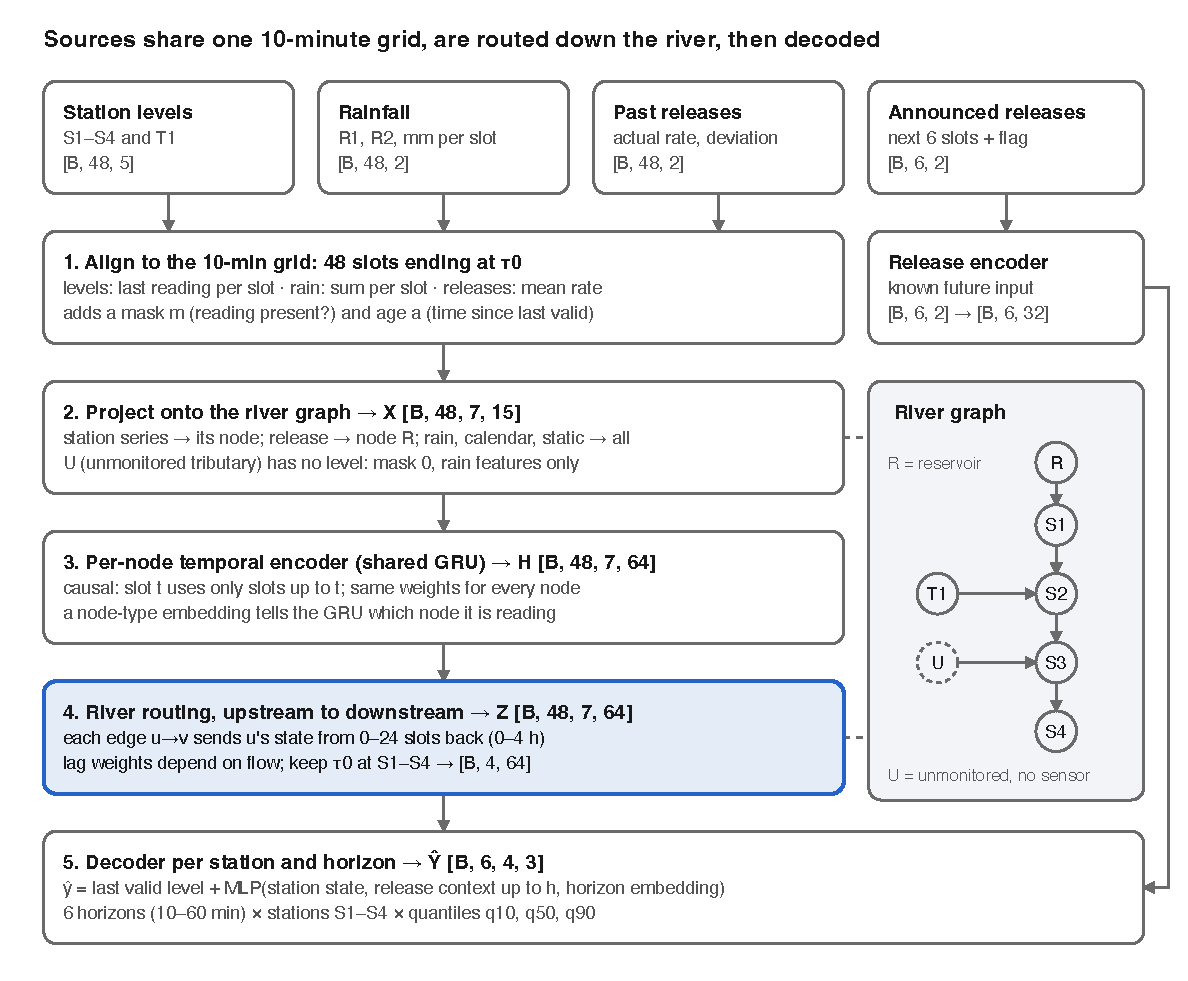
\includegraphics[width=\linewidth]{figures/q1_architecture.pdf}
\caption*{Figure Q1.1. System architecture.}
\end{figure}

Every source is first put on the same 48 ten-minute slots, then attached to its node on the river graph. The graph state is decoded per station and horizon together with the announced releases.

Axes: B = issuance times in a batch, 48 = history slots, 7 = graph nodes, 15 = features per node, 64 = hidden width, 6 = horizons, 4 = stations, 3 = quantiles.

\begin{itemize}
\tightlist
\item
  \textbf{Alignment} (step 1) turns readings with different timing into one grid.
\item
  \textbf{Projection} (step 2) reshapes station-indexed and gauge-indexed tensors into one node-indexed tensor.
\item
  \textbf{Selection} (end of step 4) keeps the issuance slot and the four forecast stations.
\end{itemize}

\subsection*{2. Assumptions}

The design rests on ten assumptions. Each one fills a gap the brief leaves open, and each can be checked against historical data before deployment.

\textbf{Supplied facts (not assumptions).}

\begin{itemize}
\tightlist
\item
  Levels at S1--S4 and T1 every 10 minutes.
\item
  Rainfall at R1 and R2, with timestamps and gauge locations.
\item
  Recorded reservoir releases, plus future schedules announced before issuance, with their announcement and effective times.
\item
  Station locations, river connectivity and distances along the river.
\item
  The monitored tributary joins between S1 and S2, and the unmonitored tributary between S2 and S3.
\item
  Travel times and unmonitored inflows are not supplied. Future rain and future levels are unknown at issuance.
\end{itemize}

{\def\LTcaptype{none} % do not increment counter
\begin{longtable}[]{@{}
  >{\raggedright\arraybackslash}p{(\linewidth - 6\tabcolsep) * \real{0.0640}}
  >{\raggedright\arraybackslash}p{(\linewidth - 6\tabcolsep) * \real{0.3256}}
  >{\raggedright\arraybackslash}p{(\linewidth - 6\tabcolsep) * \real{0.2791}}
  >{\raggedright\arraybackslash}p{(\linewidth - 6\tabcolsep) * \real{0.3314}}@{}}
\toprule\noalign{}
\begin{minipage}[b]{\linewidth}\raggedright
ID
\end{minipage} & \begin{minipage}[b]{\linewidth}\raggedright
Assumption
\end{minipage} & \begin{minipage}[b]{\linewidth}\raggedright
Why it is reasonable
\end{minipage} & \begin{minipage}[b]{\linewidth}\raggedright
Effect on the design
\end{minipage} \\
\midrule\noalign{}
\endhead
\bottomrule\noalign{}
\endlastfoot
A1 & At least 3 years of 10-minute history, including several high-water events. & Authorities typically archive telemetry for years; one year would miss seasonal regimes. & Split by year into train, validation and test. Model size (about 150k parameters) suits this amount of data. \\
A2 & Readings usually arrive within 20 minutes; occasional outages last up to several hours. & Typical of radio or cellular telemetry. & Inputs are rebuilt as available at issuance, and training simulates delays and outages (Section 5). \\
A3 & Level sensors have about ±1--2 cm noise, with occasional spikes and flatlines; tipping-bucket gauges under-read intense rain. & Common failure modes of these sensors. & A quality check turns spikes and flatlines into missing values. Rain is an input, not a target, and uncertainty bands absorb the bias. \\
A4 & All timestamps share one clock (UTC); readings may sit off the 10-minute mark. & Off-grid readings are common; a shared clock is standard. & Each series is resampled onto a grid ending at the issuance time τ0. \\
A5 & Flow only moves downstream: no backwater from the town reach and no tidal effect. Each station has a stable level--discharge relation. & The site is a mountain river with no tidal influence. & Directed graph with edges pointing downstream only. Levels are modelled directly, without discharge conversion. \\
A6 & Total travel time from the reservoir to S4 is at most 4 hours, so no single reach takes longer; travel is shorter at high flow. & The stations are a few kilometres apart; flood waves move faster when the river is high. & Each edge looks up to 24 slots (4 h) back, with lag weights that depend on the current state. The 8-hour window is twice the longest total delay. \\
A7 & Rain affects levels after 30 minutes to 6 hours. R1 represents the upper catchment and R2 the catchment of the unmonitored tributary, as on the site map. & Small mountain catchments respond within hours. & 8-hour history window. Both gauges feed every node with learned weights, and R2 mainly drives U. \\
A8 & Recorded releases are accurate actual flows. Announcements cover at least the next hour, and releases change in steps. & Release gates are metered and scheduled by operators. & Past slots use recorded actuals; future slots use the latest announcement (Section 5). \\
A9 & The unmonitored tributary is the only significant unmeasured inflow, and it is driven by rain plus baseflow. & It is the only one shown on the site map; abstractions are assumed small. & A latent node U carries this inflow. The residual of S3 against S2 teaches the model its size. \\
A10 & Channel geometry, rating relations and operating rules stay stable over the record. & No major works are mentioned. & One model is trained on the whole record, with retraining after a flood that reshapes the bed or a datum change. \\
\end{longtable}
}

\subsection*{3. Forecasting task and data specification}

At each issuance time τ0 (every 10 minutes, on the :00, :10, \ldots{} mark) the system reads the last 8 hours and outputs six 10-minute steps of level at S1--S4. The required one-hour forecast is step h = 6. Steps 1--5 come at no extra cost and give extra training signal.

\begin{itemize}
\tightlist
\item
  \textbf{Time step:} Δ = 10 min.
\item
  \textbf{History window:} L = 48 slots, from τ0 − 470 min to τ0. Slot t covers (t − 10 min, t{]}. Eight hours is twice the longest assumed reservoir-to-S4 travel time (A6) and covers the rain response (A7).
\item
  \textbf{Horizon:} h = 1\ldots6, i.e.~τ0 + 10 \ldots{} τ0 + 60 min.
\item
  \textbf{Outputs:} level at S1--S4 for each horizon, as three quantiles (q10, q50, q90). q50 is the point forecast.
\item
  \textbf{Batch axis B:} independent issuance times. In training, B windows are sampled from the training years; in operation, B = 1.
\end{itemize}

{\def\LTcaptype{none} % do not increment counter
\begin{longtable}[]{@{}
  >{\raggedright\arraybackslash}p{(\linewidth - 10\tabcolsep) * \real{0.0797}}
  >{\raggedright\arraybackslash}p{(\linewidth - 10\tabcolsep) * \real{0.0942}}
  >{\raggedright\arraybackslash}p{(\linewidth - 10\tabcolsep) * \real{0.0942}}
  >{\raggedright\arraybackslash}p{(\linewidth - 10\tabcolsep) * \real{0.2971}}
  >{\raggedright\arraybackslash}p{(\linewidth - 10\tabcolsep) * \real{0.0870}}
  >{\raggedright\arraybackslash}p{(\linewidth - 10\tabcolsep) * \real{0.3478}}@{}}
\toprule\noalign{}
\begin{minipage}[b]{\linewidth}\raggedright
Tensor
\end{minipage} & \begin{minipage}[b]{\linewidth}\raggedright
Role
\end{minipage} & \begin{minipage}[b]{\linewidth}\raggedright
Shape
\end{minipage} & \begin{minipage}[b]{\linewidth}\raggedright
Axes
\end{minipage} & \begin{minipage}[b]{\linewidth}\raggedright
Time coverage
\end{minipage} & \begin{minipage}[b]{\linewidth}\raggedright
Content
\end{minipage} \\
\midrule\noalign{}
\endhead
\bottomrule\noalign{}
\endlastfoot
Y\_obs & input & {[}B, 48, 5{]} & batch, history slot, station (S1, S2, S3, S4, T1) & τ0 − 470 \ldots{} τ0 & Level in m, standardised per station, last reading carried forward \\
M & input & {[}B, 48, 5{]} & same as Y\_obs & same & 1 if a valid reading for the slot had arrived by τ0, else 0 \\
A & input & {[}B, 48, 5{]} & same as Y\_obs & same & Age: hours since the station's last valid reading \\
P & input & {[}B, 48, 2{]} & batch, slot, gauge (R1, R2) & same & Rain in mm per slot (sum of readings in the slot); missing slots masked \\
Q\_past & input & {[}B, 48, 2{]} & batch, slot, (actual release, actual − scheduled) & same & Recorded release rate in m³/s and its deviation from the schedule \\
C & input (calendar) & {[}B, 48, 4{]} & batch, slot, (sin and cos of hour-of-day, sin and cos of day-of-year) & same & Time features from each slot's timestamp: daily release schedules, seasonal snowmelt and baseflow \\
Q\_fut & input (known future) & {[}B, 6, 2{]} & batch, future slot, (announced rate, announced flag) & τ0 + 10 \ldots{} τ0 + 60 & Latest release announced at or before τ0 for each slot; flag 0 means none announced, current rate held \\
S & input (static) & {[}7, 4{]} & node, (distance from reservoir in km, node type id, observed flag, catchment flag) & constant & Fixed site facts \\
X & model input after projection & {[}B, 48, 7, F{]} & batch, slot, graph node (R, S1, T1, S2, U, S3, S4), feature & τ0 − 470 \ldots{} τ0 & Per node: value, mask, age, P (both gauges), release features (R only), calendar and static features. F = 15 (value, mask, age, 2 rain, 2 release, 4 calendar, 4 static) \\
Ŷ & output & {[}B, 6, 4, 3{]} & batch, horizon, station (S1--S4), quantile (q10, q50, q90) & τ0 + 10 \ldots{} τ0 + 60 & Forecast level in m \\
Y, M\_Y & training target & {[}B, 6, 4{]} & batch, horizon, station & τ0 + 10 \ldots{} τ0 + 60 & Observed future level and its valid mask; never an input \\
\end{longtable}
}

\textbf{Alignment across sampling times.} Every series is put on the same 48 slots ending at τ0.

\begin{itemize}
\tightlist
\item
  Levels take the latest reading inside each slot.
\item
  Rain takes the sum of readings in the slot.
\item
  Releases take the time-weighted mean rate over the slot, from the recorded effective times.
\item
  Announced releases are placed by their effective time into the six future slots.
\end{itemize}

\textbf{Alignment across locations.} Each station's series becomes the feature vector of its graph node. The reservoir release becomes node R. Rain from both gauges and the calendar features C are copied to every node, and learned weights decide which gauge matters where. Node U has no level reading, so its mask is always 0 and only rain and static features reach it.

\textbf{Available at issuance:} readings with arrival time ≤ τ0, recorded releases up to τ0, and announcements made at or before τ0.

\textbf{Not available at issuance:} future rain, future levels, unannounced release changes, and readings still in transit. Training windows are rebuilt with the same cut-off, so the model never learns from data it will not have in operation.

\subsection*{4. Model computations and design justification}

The forecaster is a shared GRU per node, followed by one downstream sweep of lagged messages along the river graph and a decoder that predicts the change from the last observed level. Physics sets the graph, the direction of flow and the time ordering; the network learns lags, magnitudes and rain response.

\begin{figure}[H]\centering
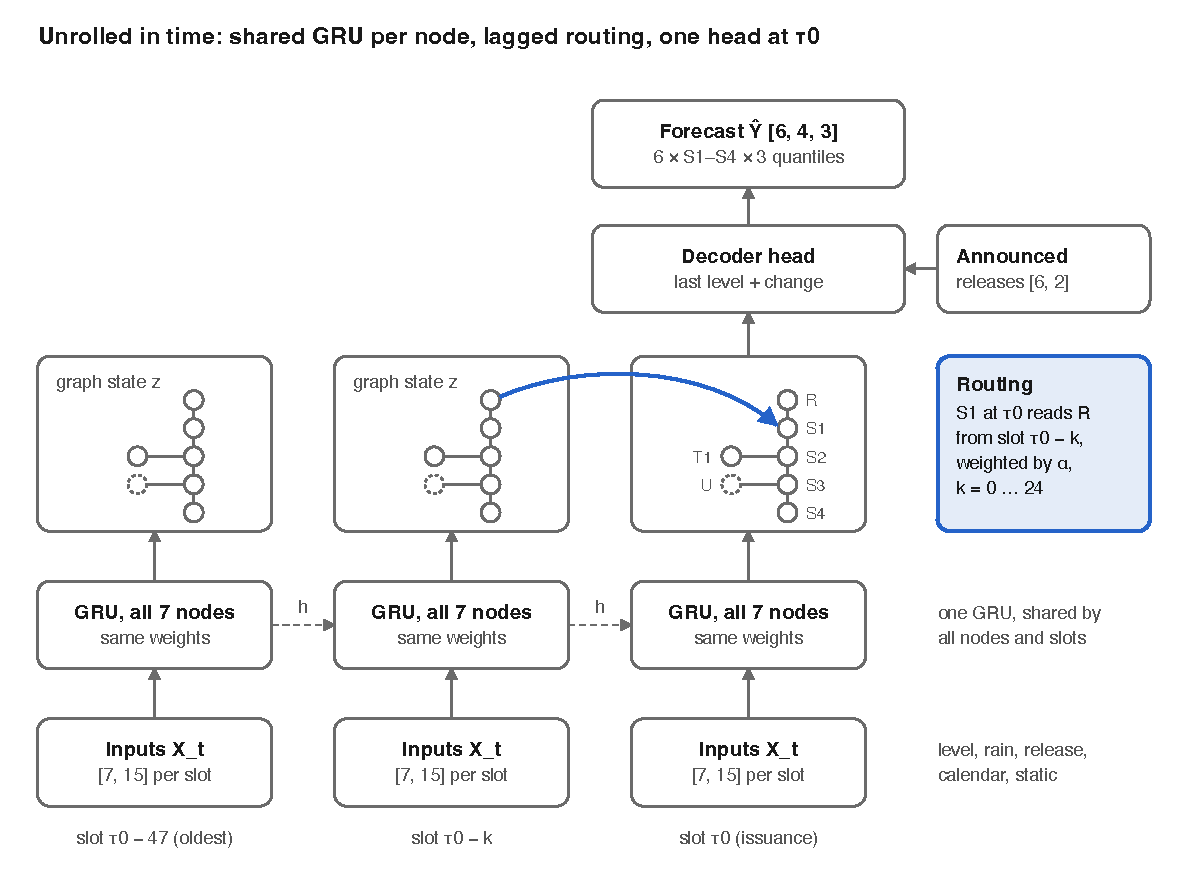
\includegraphics[width=\linewidth]{figures/q1_unrolled.pdf}
\caption*{Figure Q1.2. The model unrolled over the 48 history slots.}
\end{figure}

Each column is one 10-minute slot. The same GRU updates every node's state from its own inputs, the routing step pulls upstream states from earlier slots (accent arrow), and only the issuance slot τ0 feeds the decoder.

\textbf{Notation.}

\begin{itemize}
\tightlist
\item
  Nodes V = \{R, S1, T1, S2, U, S3, S4\}.
\item
  Edges E = \{R→S1, S1→S2, T1→S2, S2→S3, U→S3, S3→S4\}.
\item
  \(x_v^t \in \mathbb{R}^F\) is node v's feature vector at slot t (Section 3), and \(s_v\) its static features.
\item
  ỹ\_v is v's last valid level. h = 1\ldots6 is the horizon, and q ∈ \{0.1, 0.5, 0.9\} a quantile.
\item
  d = 64 is the hidden width.
\end{itemize}

\textbf{Block 1. Encoding and temporal encoder} (one GRU, weights shared by all nodes):

\[
e_v^t = W_{in}\,x_v^t + E_{type}[v] + W_s\,s_v, \qquad h_v^t = \mathrm{GRU}\big(e_v^t,\; h_v^{t-1}\big), \quad h_v^{\tau_0-L} = 0
\]

\textbf{Block 2. River routing with learned travel times.} Nodes are processed in downstream order R, T1, U, S1, S2, S3, S4, so one sweep carries reservoir information all four hops to S4. For each edge u→v and lag k = 0\ldots K, with K = 24 slots (4 h):

\[
\begin{gathered}
\alpha_{uv,k}^t = \operatorname{softmax}_k\!\Big(b_{uv,k} + w_{uv}^{\top}\,[\,h_v^t \,;\, z_u^t\,]\Big) \\ m_{u\to v}^t = \sum_{k=0}^{K} \alpha_{uv,k}^t\, W_{uv}\, z_u^{t-k}
\end{gathered}
\]

\[
z_v^t = h_v^t + \mathrm{MLP}_{node}\Big(\big[\,h_v^t \,;\, \textstyle\sum_{u:(u,v)\in E} m_{u\to v}^t\,\big]\Big), \qquad z_v^t = h_v^t \text{ for sources } R,\,T1,\,U
\]

The lag weights α depend on both nodes' current state, so the peak of α shifts to shorter lags when the river is high (A6). Lags that point before the first history slot (t − k \textless{} τ0 − 47) are masked out of the softmax. Chained lags along the four reaches could add up to more than 48 slots, but under A6 the real reservoir-to-S4 delay is at most 24 slots, so the window covers every physically plausible path.

\textbf{Block 3. Known future releases.} Each announced slot is embedded, then each station collects only releases effective up to its horizon:

\[
c^j = \mathrm{MLP}_q\big(\hat q_{\tau_0+j\Delta},\, f_{\tau_0+j\Delta}\big), \qquad r_{v,h} = \sum_{j=1}^{h} \beta_{v,\,h-j}\; c^j
\]

\textbf{Block 4. Forecast mapping.} The decoder predicts the change from the last valid level. Quantiles are kept ordered with softplus offsets:

\[
\begin{gathered}
\hat y_{v,h,0.5} = \tilde y_v + g_\theta\big([\,z_v^{\tau_0} ; r_{v,h} ; E_h[h]\,]\big) \\ \hat y_{v,h,0.9} = \hat y_{v,h,0.5} + \operatorname{softplus}(u^{+}_{v,h}) \\ \hat y_{v,h,0.1} = \hat y_{v,h,0.5} - \operatorname{softplus}(u^{-}_{v,h})
\end{gathered}
\]

\textbf{Training objective.} A masked, flood-weighted pinball loss over stations, horizons and quantiles:

\[
\begin{gathered}
\mathcal{L} = \frac{1}{\sum m}\sum_{b,v,h} m_{b,v,h}\,\omega_{b,v,h} \sum_{q} \rho_q\big(y_{b,v,h} - \hat y_{b,v,h,q}\big) \\ \rho_q(e) = \max\big(q\,e,\,(q-1)\,e\big) \\ \omega = 1 + \lambda\,\mathbf{1}[\,y > y_{watch}\,]
\end{gathered}
\]

Here m masks targets that were never observed. y\_watch is the flood-watch level and λ = 4, so high water, which matters most for preparedness, is not drowned out by calm days.

\textbf{Nowcast head.} The fallback anchor used in Section 5(i), \(\hat y_{v,0} = \mathrm{MLP}_{now}(z_v^{\tau_0})\), is trained alongside \(\mathcal{L}\) with a masked L1 loss on the current level. During this loss the station's own readings from the last 60 minutes are hidden from the input, so the head learns to work without them:

\[
\begin{gathered}
\mathcal{L}_{now} = \frac{1}{\sum m_0}\sum_{b,v} m_{b,v,0}\,\big|\,y_{b,v}(\tau_0) - \hat y_{b,v,0}\big| \\ \mathcal{L}_{total} = \mathcal{L} + 0.1\,\mathcal{L}_{now}
\end{gathered}
\]

Training uses every 10-minute issuance in the training years, with inputs cut off as available at issuance. Inputs are randomly masked: 10\% of single slots, plus whole-station blackouts of 1--6 h. Training uses Adam with early stopping on the validation year; the test year is reported once. Baselines use the same splits: persistence (ŷ = ỹ); NLinear and DLinear per station, the lecture's simple linear baselines; a VAR whose coefficients are masked by the river adjacency, the classical operator for graphs; and a per-station GRU without routing, which removes Block 2.

\textbf{Physical relations versus learned mappings.}

{\def\LTcaptype{none} % do not increment counter
\begin{longtable}[]{@{}
  >{\raggedright\arraybackslash}p{(\linewidth - 4\tabcolsep) * \real{0.1667}}
  >{\raggedright\arraybackslash}p{(\linewidth - 4\tabcolsep) * \real{0.4615}}
  >{\raggedright\arraybackslash}p{(\linewidth - 4\tabcolsep) * \real{0.3718}}@{}}
\toprule\noalign{}
\begin{minipage}[b]{\linewidth}\raggedright
Element
\end{minipage} & \begin{minipage}[b]{\linewidth}\raggedright
Fixed by physics (assumption)
\end{minipage} & \begin{minipage}[b]{\linewidth}\raggedright
Learned from data
\end{minipage} \\
\midrule\noalign{}
\endhead
\bottomrule\noalign{}
\endlastfoot
Who affects whom & Directed river graph, downstream only (A5) & Strength of each edge (W\_uv, MLP\_node) \\
Travel time & Causal, at most 4 h from reservoir to S4 (A6) & Lag weights α, which depend on state \\
Confluences & T1 joins at S2, U at S3 & Each inflow's contribution \\
Rainfall & Acts with delay through the catchments (A7) & Response per node and gauge \\
Reservoir & Enters at R, reaches S1 first (A8) & Effect size and timing \\
Short-term level & Persistence anchor ỹ\_v & Change over 10--60 min \\
\end{longtable}
}

\textbf{How each source reaches each forecast.}

{\def\LTcaptype{none} % do not increment counter
\begin{longtable}[]{@{}
  >{\raggedright\arraybackslash}p{(\linewidth - 8\tabcolsep) * \real{0.0982}}
  >{\raggedright\arraybackslash}p{(\linewidth - 8\tabcolsep) * \real{0.1161}}
  >{\raggedright\arraybackslash}p{(\linewidth - 8\tabcolsep) * \real{0.1429}}
  >{\raggedright\arraybackslash}p{(\linewidth - 8\tabcolsep) * \real{0.3661}}
  >{\raggedright\arraybackslash}p{(\linewidth - 8\tabcolsep) * \real{0.2768}}@{}}
\toprule\noalign{}
\begin{minipage}[b]{\linewidth}\raggedright
Forecast
\end{minipage} & \begin{minipage}[b]{\linewidth}\raggedright
Upstream river
\end{minipage} & \begin{minipage}[b]{\linewidth}\raggedright
Tributary
\end{minipage} & \begin{minipage}[b]{\linewidth}\raggedright
Rainfall
\end{minipage} & \begin{minipage}[b]{\linewidth}\raggedright
Reservoir release
\end{minipage} \\
\midrule\noalign{}
\endhead
\bottomrule\noalign{}
\endlastfoot
S1 & R (1 hop) & none & Both gauges directly (learned weights; R1 expected to dominate) & Past releases through R→S1; announced releases through r\_\{S1,h\} \\
S2 & S1 (lagged) & T1 through T1→S2 & Both gauges directly; R1 also through S1 and T1 & Through S1 (2 hops) \\
S3 & S2 (lagged) & U through U→S3 (latent) & Both gauges directly; R2 also through U & Through S2 (3 hops) \\
S4 & S3 (lagged) & Both, through S3 & Both gauges directly, plus through the chain & Through the whole chain (4 hops) \\
\end{longtable}
}

\textbf{Where the design sits in the lecture's taxonomy.}

\begin{itemize}
\tightlist
\item
  \textbf{Geometry: graph.} The authority supplies connectivity and distances, so space is a 7-node directed graph rather than a grid or bare channels.
\item
  \textbf{Temporal operator: recurrence.} One GRU with shared weights runs along time at every node (Block 1).
\item
  \textbf{Spatial operator: message passing with lags.} Each node reads its upstream neighbours' states from up to 24 slots back (Block 2).
\item
  \textbf{Composition: factorized, time then space.} The GRU never sees other nodes. Space and time meet in the routing step, because each message comes from an earlier slot of an upstream node. This avoids the pitfall the lecture flags for network-level factorization, where space never mixes with time, and keeps travel time as an explicit, inspectable weight α.
\item
  \textbf{Alternative considered: recurrent mixing.} As in ConvLSTM, graph messages could run inside every GRU step (a graph-convolutional GRU). It mixes more deeply but hides travel time inside the recurrence. It is our first upgrade if validation shows routing is the bottleneck.
\item
  \textbf{Rejected: joint space--time attention.} 48 × 7 = 336 tokens would be affordable, but attention would have to learn from few floods the proximity the river graph gives for free.
\end{itemize}

\textbf{Why these choices.}

\begin{itemize}
\tightlist
\item
  \textbf{Known graph instead of full attention.} With 7 nodes and known connectivity, the graph is the physics; attention would have to rediscover it from limited flood data. One downstream sweep gives S4 a path from every upstream source, the reach lesson from the companion notebook, at negligible cost. Treating the stations as bare channels, the lecture's ``channels only'' geometry, would force the model to learn from few floods a connectivity the authority already supplies.
\item
  \textbf{Learned, state-dependent lags instead of fixed delays.} Travel times are not supplied and change with flow (A6).
\item
  \textbf{Residual on the last level.} One-hour changes are small relative to the level, so the network learns only the change. This is the same idea as NLinear's subtract-the-last-value fix for non-stationary series. If it fails, the output degrades towards persistence instead of nonsense.
\item
  \textbf{Quantiles.} Flood decisions need a band, not only a number. Pinball loss gives calibrated q10 and q90 without assuming Gaussian errors. A Gaussian head trained with negative log-likelihood, the lecture's alternative, would also work, but it forces symmetric bands while flood rises are skewed.
\item
  \textbf{Shared GRU with node embeddings.} Five gauged series are too few to train a separate encoder per node; sharing weights keeps the model at about 150k parameters.
\end{itemize}

\subsection*{5. Operation and exceptional conditions}

Every run rebuilds its inputs from the database with the cut-off ``arrived by τ0'', so gaps, late data and new announcements are handled by the same input construction the model was trained on.

\textbf{(i) Missing observations.}

\begin{itemize}
\tightlist
\item
  A missing slot carries the last valid value forward with mask m = 0, and the age feature keeps counting. The model sees that the value is stale, not only that it is old.
\item
  Training rehearses this: 10\% of single slots, and whole-station blackouts of 1--6 h, are masked at random.
\item
  A station that is down still receives upstream messages, so its state is inferred from its neighbours. For example, S3 keeps a state from S2 and U.
\item
  If the forecast station's own last reading is more than 60 minutes old, the anchor ỹ\_v is replaced by a nowcast head ŷ\_\{v,0\} = MLP\_now(z\_v\^{}\{τ0\}). This head is trained to reconstruct the current level from the graph state.
\item
  The forecast is labelled ``degraded''. Its band widens automatically, because the quantile heads see the age feature.
\item
  If every station is down, the system issues persistence from the last valid readings and raises an alert.
\end{itemize}

\textbf{(ii) Delayed observations.}

\begin{itemize}
\tightlist
\item
  Each record keeps two times: measurement time and arrival time. A run at τ0 uses only records with arrival time ≤ τ0. A late reading leaves its slot masked until it arrives, and the next run, 10 minutes later, picks it up automatically.
\item
  The model holds no state between runs, so nothing needs patching.
\item
  Training windows use the logged arrival times where they exist, otherwise delays sampled from the assumed distribution (A2).
\item
  Issued forecasts are not revised. If late data moves q50 by more than 5 cm at any station, an updated forecast is issued at the next 10-minute run, as usual.
\end{itemize}

\textbf{(iii) Announced future releases.}

\begin{itemize}
\tightlist
\item
  Announcements are stored with announcement time and effective time. For each of the six future slots, Q\_fut takes the latest announcement made at or before τ0 that is in force in that slot.
\item
  With no announcement, the current rate is held and the flag is 0, so the model can learn that unannounced periods are less certain.
\item
  In training, Q\_fut is rebuilt from the announcements known at each historical issuance time, never from the releases that actually happened. Otherwise the model would learn to trust schedules more than it should.
\item
  A release enters a station's forecast only through r\_\{v,h\}, which sums slots effective up to horizon h. A release scheduled for minute 50 cannot change the 20-minute forecast.
\end{itemize}

\textbf{(iv) Scheduled versus actual releases.}

\begin{itemize}
\tightlist
\item
  Past slots always use the recorded actual release. Q\_past also carries the deviation from the schedule (actual − scheduled), so the model learns how reliable announcements have recently been.
\item
  Future slots must use the schedule. When the actual release departs from it, the first signal is the release record (if it is real-time), otherwise the S1 level. The next run, 10 minutes later, corrects the forecast through Q\_past and the routing.
\item
  Quantile bands for S1 and S2 widen when recent deviations are non-zero, because the deviation is an input to the quantile heads.
\item
  Large deviations (above 20\% of the scheduled rate) are flagged to operators alongside the forecast.
\end{itemize}

\textbf{Running every 10 minutes is feasible.}

\begin{itemize}
\tightlist
\item
  One run reads about 8 hours × 7 series (under 400 readings), aligns them in milliseconds, and performs one forward pass.
\item
  The forward pass is a 48-step GRU on 7 nodes with d = 64 (about 8 million multiply-adds, roughly 17 MFLOP), plus routing over 6 edges × 25 lags: a few tens of MFLOP in total, well under 0.1 s on a single CPU core. The whole pipeline takes seconds, against a 600-second budget.
\item
  Training is offline: hours on a CPU or a single GPU. It is repeated monthly, or after a reshaping flood or a sensor change (A10).
\item
  If the model service fails, the operations system falls back to persistence forecasts, so a forecast is always issued.
\end{itemize}

\subsection*{6. Uncertainty, limitations and additional information}

The largest risks are at S3 and S4 during local rain, from the unmonitored tributary, and in floods larger than any in the record. The quantile bands carry most of this uncertainty, and the requests below would shrink it.

\textbf{Uncertainties and limitations.}

{\def\LTcaptype{none} % do not increment counter
\begin{longtable}[]{@{}
  >{\raggedright\arraybackslash}p{(\linewidth - 8\tabcolsep) * \real{0.0558}}
  >{\raggedright\arraybackslash}p{(\linewidth - 8\tabcolsep) * \real{0.1929}}
  >{\raggedright\arraybackslash}p{(\linewidth - 8\tabcolsep) * \real{0.2589}}
  >{\raggedright\arraybackslash}p{(\linewidth - 8\tabcolsep) * \real{0.2487}}
  >{\raggedright\arraybackslash}p{(\linewidth - 8\tabcolsep) * \real{0.2437}}@{}}
\toprule\noalign{}
\begin{minipage}[b]{\linewidth}\raggedright
\#
\end{minipage} & \begin{minipage}[b]{\linewidth}\raggedright
Uncertainty or limitation
\end{minipage} & \begin{minipage}[b]{\linewidth}\raggedright
Forecast impact
\end{minipage} & \begin{minipage}[b]{\linewidth}\raggedright
Our response
\end{minipage} & \begin{minipage}[b]{\linewidth}\raggedright
What remains unresolved
\end{minipage} \\
\midrule\noalign{}
\endhead
\bottomrule\noalign{}
\endlastfoot
U1 & Unmonitored tributary: its inflow is never observed & S3 and S4 under-forecast rises driven by local rain; bands are widest there & Latent node U driven by R2, learned from the residual of S3 against routed S2 & U's inflow cannot be separated from rating errors at S3; a storm missed by R2 is missed entirely \\
U2 & Travel times change with flow & Peaks arrive earlier or later than forecast at S2--S4 & State-dependent lag weights (Block 2) and an 8-hour history & Flows above the training range extrapolate the lag curve \\
U3 & Floods larger than any in the record & Peak levels at the town are likely underestimated & Flood-weighted loss, persistence anchor, wider q90 & No reliable extrapolation without a hydraulic model or longer record \\
U4 & Future rain is unknown & A storm that starts after τ0 over the lower catchment can raise S3 and S4 within the hour unseen & Bands learned from historical storms & Unresolved without a rainfall forecast (request I3) \\
U5 & Only two rain gauges & Convective cells between gauges are missed or misplaced & Both gauges feed every node; learned weights & Spatial rain coverage stays poor \\
U6 & Releases deviate from their schedule & S1 and S2 errors for 10--30 minutes after a change & Deviation feature, 10-minute correction, operator flag & Unannounced emergency releases are seen only after they happen \\
U7 & Sensor drift, datum changes, rating shifts after floods & Biased levels at one station; the model trusts wrong inputs & Quality checks, residual monitoring per station, retraining (A10) & Slow drift can go unnoticed for weeks \\
U8 & Telemetry delays and outages & Degraded forecasts with wider bands & Masks, age features, nowcast anchor (Section 5) & Long outages at S3 or S4 leave the town reach poorly constrained \\
U9 & Model limits: a learned model with no explicit mass balance & Physically inconsistent forecasts are possible, such as S4 falling while all upstream nodes rise & Persistence fallback; checks against this pattern & Not guaranteed by construction \\
\end{longtable}
}

\textbf{Additional information requests.} The system runs without any of these; each one reduces a specific uncertainty above.

{\def\LTcaptype{none} % do not increment counter
\begin{longtable}[]{@{}
  >{\raggedright\arraybackslash}p{(\linewidth - 6\tabcolsep) * \real{0.0710}}
  >{\raggedright\arraybackslash}p{(\linewidth - 6\tabcolsep) * \real{0.3290}}
  >{\raggedright\arraybackslash}p{(\linewidth - 6\tabcolsep) * \real{0.3355}}
  >{\raggedright\arraybackslash}p{(\linewidth - 6\tabcolsep) * \real{0.2645}}@{}}
\toprule\noalign{}
\begin{minipage}[b]{\linewidth}\raggedright
\#
\end{minipage} & \begin{minipage}[b]{\linewidth}\raggedright
Request to the authority
\end{minipage} & \begin{minipage}[b]{\linewidth}\raggedright
How it would help
\end{minipage} & \begin{minipage}[b]{\linewidth}\raggedright
Usable without it?
\end{minipage} \\
\midrule\noalign{}
\endhead
\bottomrule\noalign{}
\endlastfoot
I1 & Any gauging, spot flow measurements or catchment area for the unmonitored tributary; ideally a temporary gauge & Calibrates the latent node U and separates its inflow from rating errors at S3 (U1) & Yes; U stays learned only from S3 residuals \\
I2 & Rating curves (level--discharge) for S1--S4 & Allows a discharge-space mass balance (S3 ≈ routed S2 + U) as a training penalty (U1, U9) & Yes; we model levels directly \\
I3 & Weather radar or a rainfall nowcast for the next hour & Covers rain that starts after issuance (U4, U5) & Yes; added as one more future input like Q\_fut \\
I4 & Cross-sections or an existing hydraulic model, and records of historical floods & Travel time against flow, and synthetic large floods for training (U2, U3) & Yes; lags stay purely learned \\
I5 & Telemetry arrival logs and quality-control flags & Realistic delay simulation and cleaner targets (A2, A3) & Yes; delays are simulated from assumptions \\
I6 & Real-time actual release telemetry, operating rules, spillway thresholds & Earlier detection of schedule deviations (U6) & Yes; S1 levels give the signal 10--30 minutes later \\
I7 & Sensor maintenance and datum-change logs & Explains jumps and prevents training on broken data (U7) & Yes; jumps are detected statistically \\
I8 & Flood-watch and warning levels for each station and the town & Sets y\_watch in the loss and the evaluation thresholds & Yes; a high percentile of each station's record is used instead \\
\end{longtable}
}

\newpage
%=====================================================================
\section*{Question 2 --- Motion or Memory?}
\textbf{Conventions.}
{\raggedright
\begin{itemize}
  \item Code is in \texttt{Question2/}: \texttt{common.py} (data split, transformations, windows, models, metrics),
  \texttt{checks.py} (Table 1), \texttt{flow.py} (Figure 1), \texttt{train.py} (one model, one seed),
  \texttt{evaluate.py} (Tables 2--6, Figures 2--6, GIFs) and \texttt{Q2.ipynb}, which runs them in order.
  \item Videos 0--7,999 train, 8,000--8,999 validation, 9,000--9,999 test. All results use the 1,000 test videos
  except Table 1, Figure 1, parameter counts and timings; model D was chosen on the validation split.
  \item Every learned model was trained with seeds 0 and 1; table entries are mean (seed 0, seed 1). Figures, GIFs
  and per-video histograms use seed 0.
  \item Hardware: Apple M1 GPU (PyTorch 2.15.0, MPS backend, macOS 15).
\end{itemize}}
\subsection*{1. Setup}
\begin{table}[!htbp]\centering\footnotesize\setlength{\tabcolsep}{4pt}
\begin{tabular}{lll}
\toprule
Check & Expected & Yours\\
\midrule
(a) $\max|M(M(x))-x|$ & 0 & 0 (\texttt{torch.equal}: True)\\
(b) $\max|R^4(x)-x|$ & 0 & 0 (\texttt{torch.equal}: True)\\
(c) $\max|MRM(x)-R^{-1}(x)|$ & 0 & 0 (\texttt{torch.equal}: True)\\
(d) bright pixel of $M(p)$ & (7, 10, 43) & (7, 10, 43)\\
(e) bright pixel of $R(p)$ & (7, 43, 10) & (7, 43, 10)\\
(f) 1$\times$ input / target frames & 1-5 / 6-10 & 1, 2, 3, 4, 5 / 6, 7, 8, 9, 10\\
(g) 2$\times$ input / target frames & 1, 3, 5, 7, 9 / 11, 13, 15, 17, 19 & 1, 3, 5, 7, 9 / 11, 13, 15, 17, 19\\
(h) 3$\times$ input / target frames & 1, 4, 7, 10, 13 / 16, 19 & 1, 4, 7, 10, 13 / 16, 19\\
\bottomrule
\end{tabular}
\caption{Transformation and window checks.}
\end{table}

\begin{figure}[!htbp]\centering
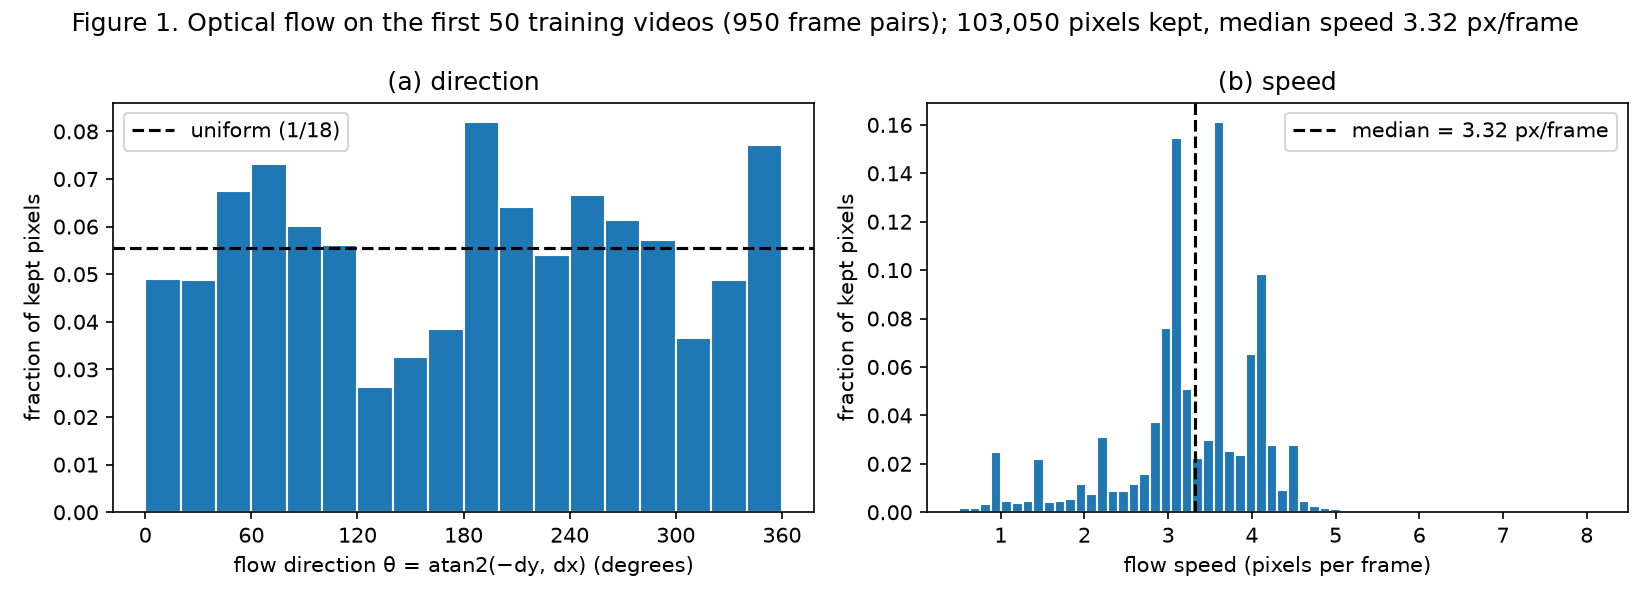
\includegraphics[width=\linewidth]{figures/fig1_flow.png}
\end{figure}

\subsection*{Q2.1}
\textbf{Direction.} Yes, mirrored and rotated trajectories should already be familiar. Figure 1(a) has no empty bins: every 20° bin holds between 2.6\% (120°--140°) and 8.2\% (180°--200°) of the kept pixels, against 5.6\% for a uniform distribution. Mirroring maps a direction θ to 180° − θ, so the mirrored histogram is Figure 1(a) reflected about 90° (the 180°--200° peak moves to 340°--360°, which already holds 7.7\%). A 90° rotation maps θ to θ + 90°, which simply shifts the histogram. Either way, every direction in the transformed videos is one the model has seen at least 2.6\% of the time. The histogram is uneven mainly because 50 videos contain only 100 digits, each moving in one direction between bounces.

\textbf{Speed.} The median speed is 3.32 px/frame, and almost all kept pixels lie between about 3 and 4.5 px/frame (peaks near 3.1, 3.6 and 4.1), with essentially nothing above 5 px/frame. At 2× the median becomes 6.64 px/frame and at 3× it becomes 9.95 px/frame, so typical motion at 2× and 3× is faster than anything in the training data.

\textbf{Overlap.} Where digits overlap, Farneback's 15-pixel window averages the motion of both digits, so those pixels get a blended direction and usually a smaller speed. This adds some weight to the low-speed tail and to directions between the two digits' true directions. It cannot change the answer: overlap does not create directions that are not there, and biasing speeds downward only widens the gap between the training speeds and 2× or 3×.


\subsection*{Q2.2}
\begin{itemize}
\item
  \textbf{Mirror:} changes digit appearance (a mirrored 2 is not a digit) but keeps speed, and it only reflects directions within a range the training data already covers (Q2.1). In practice it changes appearance only.
\item
  \textbf{Rotation:} the same, with a stronger change in appearance, since vertical strokes become horizontal for every digit. The motion statistics are again familiar.
\item
  \textbf{Speed-up:} keeps every digit's appearance (the frames themselves are untouched) but multiplies the displacement between frames by k, so it changes the motion statistics only.
\end{itemize}

This makes a controlled experiment because each transformation moves one factor while holding the other fixed, and all three keep the scene physically valid, so the correct answer T(Y) is known exactly. A model that has learned the motion rule should pass all three. If it fails mirror and rotation but not speed, the problem is appearance; if it fails speed but not mirror and rotation, the problem is motion.


\newpage
\subsection*{2. Baseline: ConvLSTM}
\begin{table}[!htbp]\centering\footnotesize\setlength{\tabcolsep}{4pt}
\begin{tabular}{llllllll}
\toprule
Model & MSE$_1$ & MSE$_2$ & MSE$_3$ & MSE$_4$ & MSE$_5$ & $E^{(5)}$ & params\\
\midrule
A & \makecell[l]{0.0171\\{\scriptsize(0.0176, 0.0166)}} & \makecell[l]{0.0205\\{\scriptsize(0.0210, 0.0199)}} & \makecell[l]{0.0227\\{\scriptsize(0.0233, 0.0221)}} & \makecell[l]{0.0245\\{\scriptsize(0.0251, 0.0239)}} & \makecell[l]{0.0262\\{\scriptsize(0.0267, 0.0256)}} & \makecell[l]{0.0222\\{\scriptsize(0.0227, 0.0216)}} & 480{,}784\\
Blank & 0.0426 & 0.0426 & 0.0426 & 0.0425 & 0.0425 & 0.0426 & 0\\
Copy-last & 0.0492 & 0.0604 & 0.0669 & 0.0708 & 0.0732 & 0.0641 & 0\\
\bottomrule
\end{tabular}
\caption{Per-horizon test MSE (mean (seed 0, seed 1) for model A).}
\end{table}

\begin{figure}[!htbp]\centering
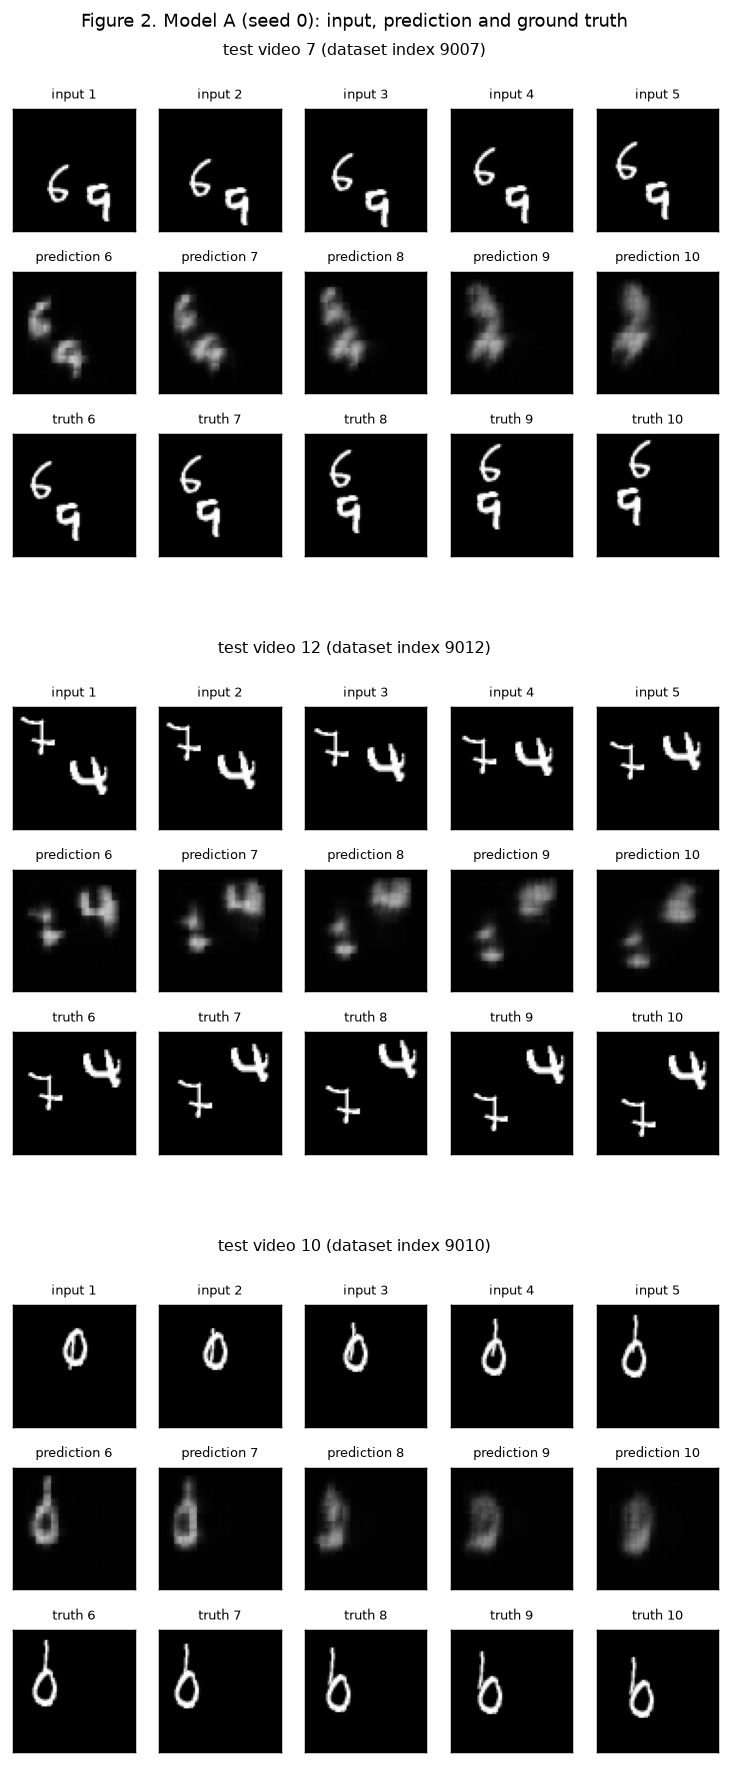
\includegraphics[height=0.8\textheight]{figures/fig2_predictions.png}
\end{figure}

\subsection*{Q2.3}
\textbf{Model A's reach is 8 original pixels per time step.}

\begin{itemize}
\item
  After \texttt{pixel\_unshuffle(x,\ 4)} each position of the 16×16 grid is one 4×4 patch, so moving one grid cell moves 4 original pixels.
\item
  A 3×3 convolution (stride 1, padding 1) lets each output cell see its immediate neighbours, so one pass moves information by at most 1 cell = 4 px.
\item
  Within one step τ the only spatial operations are the two gate convolutions. Everything else (the sigmoids, tanh, the elementwise cell update c, the 1×1 output convolution and the pixel shuffles) acts on one position at a time.
\item
  Possible paths to \(\hat{x}_{\tau+1}\):

  \begin{itemize}
  \tightlist
  \item
    from the new input \(u_\tau\): layer-1 convolution (1 cell), then layer-2 convolution on \(h^{(1)}_{\tau}\) (1 cell) = 2 cells;
  \item
    from \(h^{(1)}_{\tau-1}\): it enters the same layer-1 convolution as \(u_\tau\), so again 2 cells;
  \item
    from \(h^{(2)}_{\tau-1}\): only the layer-2 convolution, 1 cell.
  \end{itemize}
\item
  The cell states \(c^{(1)}\) and \(c^{(2)}\) are updated elementwise, so a path that starts in \(c^{(1)}_{\tau-1}\) passes through at most the layer-2 convolution (1 cell), and one that starts in \(c^{(2)}_{\tau-1}\) through none. They do not change the answer.
\item
  The longest path is 2 cells × 4 px = \textbf{8 px} centre-to-centre along a row or column. Along a diagonal the same 2 cells reach \(2\sqrt{2} \times 4 \approx 11.3\) px in straight-line distance. Flow speeds are straight-line distances, so I use the conservative 8 px when comparing reach with speed.
\end{itemize}

The recurrence does not add reach within one step, since states pass to the next step without any spatial mixing. It does let information keep travelling another 8 px at every step, so over the 5 input steps the network can integrate motion over a larger area, but it can link a digit's old position (in the state) to its new position (in the input) only within 8 px per update.


\subsection*{Q2.4}
\textbf{Against the references.} Model A has \(E^{(5)}\) = 0.0222 (0.0227, 0.0216), about half of Blank (0.0426) and a third of Copy-last (0.0641), and it beats both at every horizon. Copy-last is even worse than Blank because a digit drawn in the wrong place is penalised twice: once where it is drawn and once where it should be. So model A is not just copying frames; it moves the digits.

\textbf{Over the horizons.} Model A's error rises from MSE\(_1\) = 0.0171 to MSE\(_5\) = 0.0262 (+53\%), with each step adding a little less (+0.00338, +0.00225, +0.00179, +0.00167). Blank stays flat at 0.0426, and Copy-last grows faster (0.0492 to 0.0732) as the digits move further from where it left them. Figure 2 shows why model A's error grows: the digits sit roughly in the right places but get blurrier with every step, and by frame 10 they are grey blobs. Under squared error, a blurred digit is the safest guess when the position is uncertain, and the model then feeds its own blurry predictions back as input.

\textbf{Overlap.} In test video 7 the 6 moves up towards the 9, and the predictions merge the two into one vertical smear by frames 8--10 instead of keeping two digits. In test video 10 the two digits overlap almost completely at the start; the model predicts a single blob, and the second digit's stroke disappears by frame 8. When digits overlap, model A loses the separate identity of each one.


\subsection*{Q2.5}
\textit{(included exactly as first written)}

\textbf{Mirror --- partial pass.} Figure 1(a) shows flow in every direction (all 18 bins are occupied, between about 0.026 and 0.082), so mirrored trajectories (θ → 180° − θ) are familiar motion. Mirrored digits are unfamiliar shapes, though. I expect model A to move the mirrored digits to roughly the right places but to render them less sharply, so \(C_M\) and \(E_M\) will be small but clearly above zero, with \(E_M\) somewhat larger than \(E^{(5)}\).

\textbf{Rotation --- weaker pass than mirror.} A 90° rotation (θ → θ + 90°) also maps onto directions seen in training, so the motion should still be familiar. Rotated digits are further from anything in training than mirrored ones (a rotated 1 is a horizontal bar). I therefore predict \(C_R\) \textgreater{} \(C_M\) and \(E_R\) \textgreater{} \(E_M\), with the extra error coming from appearance rather than from the motion.

\textbf{Speed --- degrades at 2×, breaks down at 3×.} Model A's reach is 8 px per step (two 3×3 convolutions, each moving one 4-pixel cell). The median speed is 3.3 px/frame, so 2× ≈ 6.6 px is inside the reach but close to its edge, and the fastest digits (≈ 5 px/frame at 1×) exceed it. 3× ≈ 10 px/frame is beyond the reach for most digits. I predict \(E^{(2)}\) rises noticeably at 2×, and that at 3× the predictions fall apart: digits blur, stall near their last position or vanish, giving errors close to or worse than Copy-last.


\newpage
\subsection*{3. Testing the Baseline}
\textbf{Mirror and rotation.}
\begin{table}[!htbp]\centering\footnotesize\setlength{\tabcolsep}{4pt}
\begin{tabular}{llllll}
\toprule
Model & $E^{(5)}$ & $C_M$ & $E_M$ & $C_R$ & $E_R$\\
\midrule
A & \makecell[l]{0.0222\\{\scriptsize(0.0227, 0.0216)}} & \makecell[l]{0.00193\\{\scriptsize(0.00199, 0.00187)}} & \makecell[l]{0.0228\\{\scriptsize(0.0234, 0.0222)}} & \makecell[l]{0.00317\\{\scriptsize(0.00318, 0.00316)}} & \makecell[l]{0.0239\\{\scriptsize(0.0244, 0.0234)}}\\
Blank & 0.0426 & 0 & 0.0426 & 0 & 0.0426\\
Copy-last & 0.0641 & 0 & 0.0641 & 0 & 0.0641\\
\bottomrule
\end{tabular}
\caption{Error and consistency under mirror (M) and rotation (R), 1$\times$, t = 1.}
\end{table}

\begin{figure}[!htbp]\centering
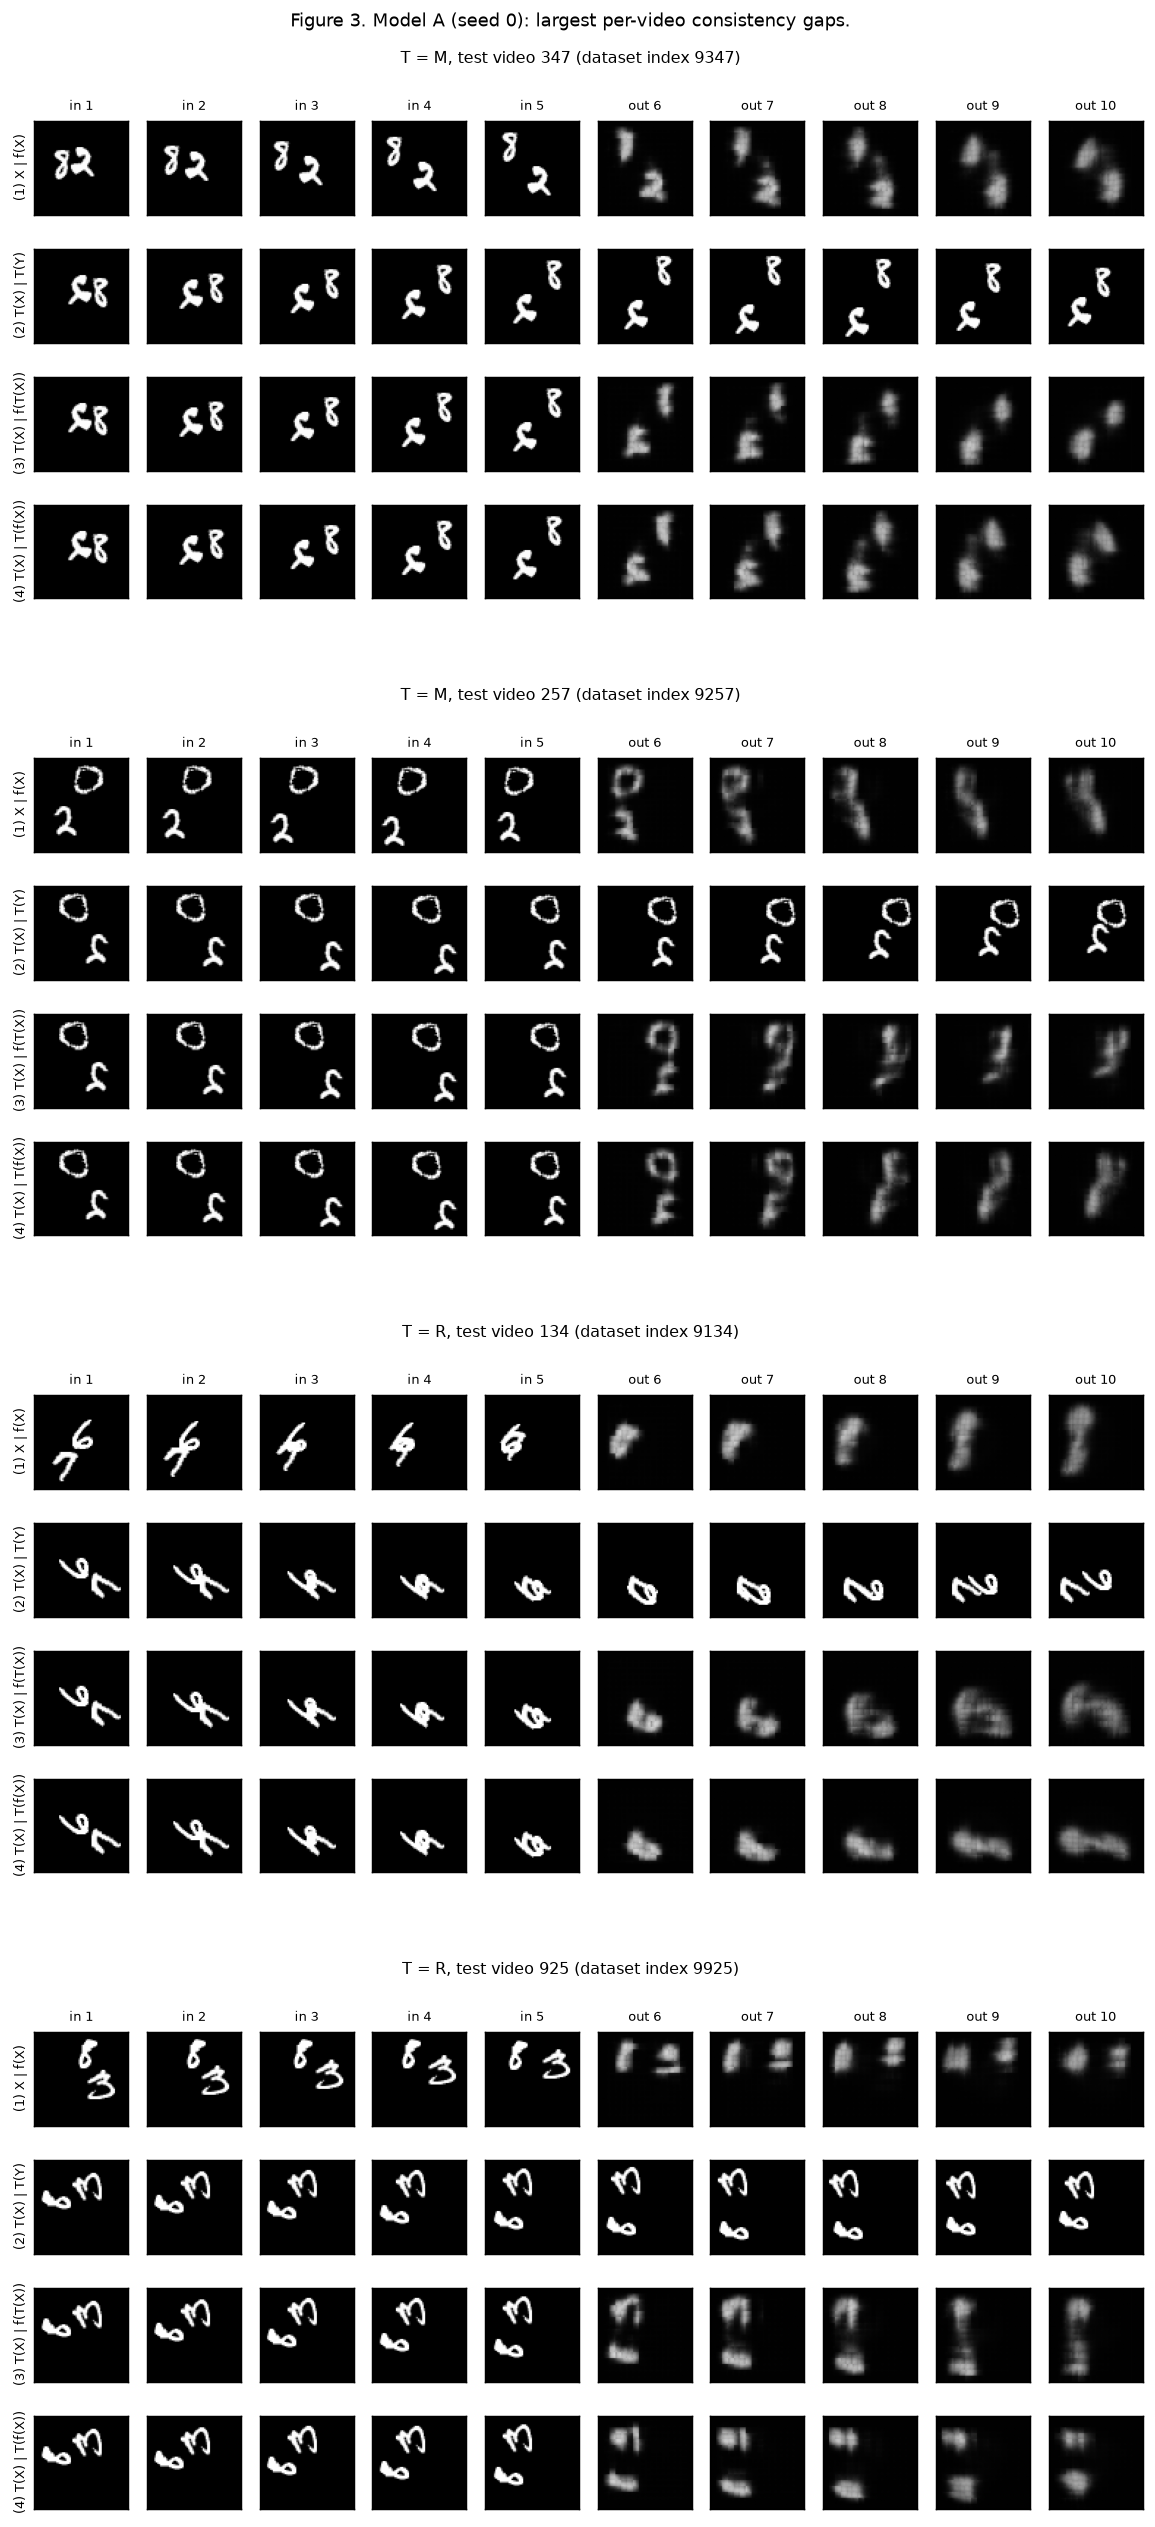
\includegraphics[height=0.82\textheight]{figures/fig3_consistency.png}
\caption*{\footnotesize GIFs: \texttt{Question2/results/gifs/fig3\_M\_video257.gif}, \texttt{Question2/results/gifs/fig3\_M\_video347.gif}, \texttt{Question2/results/gifs/fig3\_R\_video134.gif}, \texttt{Question2/results/gifs/fig3\_R\_video925.gif}}
\end{figure}

\begin{figure}[!htbp]\centering
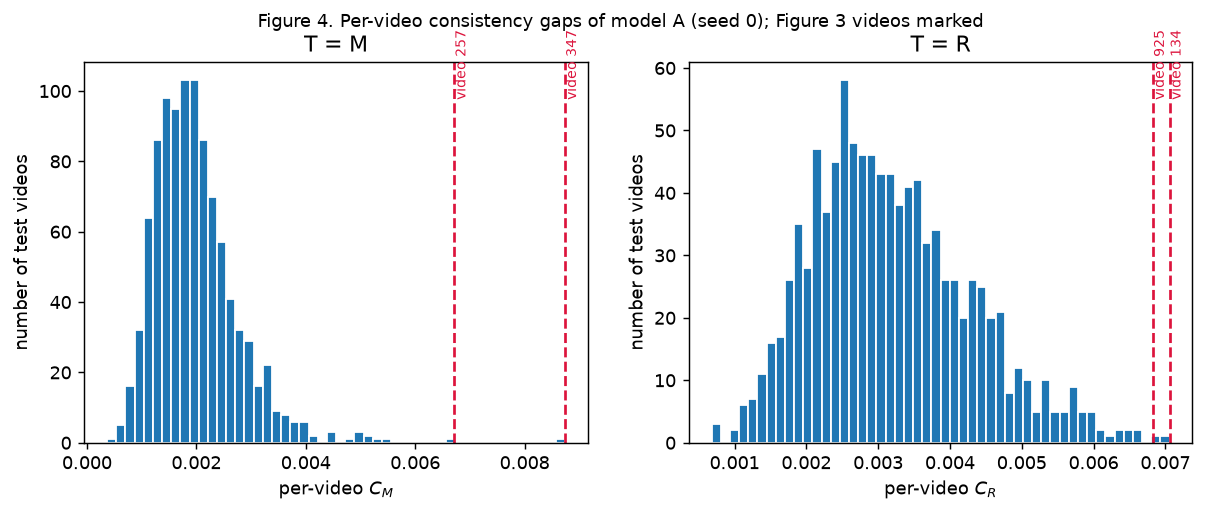
\includegraphics[width=\linewidth]{figures/fig4_consistency_hist.png}
\end{figure}

\subsection*{Q2.6}
Blank and Copy-last have \(C_M\) = \(C_R\) = 0 but \(E_M\) = \(E_R\) = 0.0426 and 0.0641, both worse than model A. A forecaster that ignores the motion (outputs nothing, or repeats the last frame) commutes with any pixel rearrangement, so it is perfectly consistent and still wrong. A small \(C_T\) therefore cannot tell ``moves things correctly in every orientation'' apart from ``does not really move things at all''; a model that blurs everything towards a blank frame would also score well. \(E_T\) measures what we actually want, whether the transformed prediction matches the transformed truth, so \(C_T\) is only meaningful next to \(E_T\) (and next to \(E^{(5)}\) on the original clips).


\subsection*{Q2.7}
\textbf{Test video 925, rotation (second-largest per-video \(C_R\), 0.00683; per-video \(E_R\) 0.0357 against the test mean of 0.0239).} In the original video an 8 and a 3 sit side by side near the top and barely move. After rotation they are stacked vertically: the rotated 3 at the top and the rotated 8 at the lower left. In the truth (row 2) the two stay well apart for all five future frames.

\begin{itemize}
\item
  \textbf{Row 4, T(f(X)):} model A's prediction on the original video, rotated. It keeps two separate blobs, one above the other, through frame 10. The layout is right and the digits are just blurred.
\item
  \textbf{Row 3, f(T(X)):} what model A predicts when it sees the rotated video. The top digit loses its shape and becomes a tall vertical smear that stretches downward, while the lower digit stays a blob. By frames 9--10 the gap between them has closed and they form one vertical streak.
\end{itemize}

So in the rotated scene the model's account of the motion changes from ``two digits staying apart'' to ``the top digit drifting down into the bottom one''. The upper digit is effectively lost into the lower one, even though the true motion is the same as in the original video turned by 90°.


\subsection*{Q2.8}
Yes. Model A's rotation gap is larger than its mirror gap for both seeds: \(C_R\) = 0.00317 against \(C_M\) = 0.00193 (about 1.6 times larger), and \(E_R\) = 0.0239 against \(E_M\) = 0.0228, with \(E^{(5)}\) = 0.0222. Figure 4 shows the same thing: the per-video \(C_R\) histogram is wider and sits further right than the \(C_M\) histogram.

The difference comes from appearance, not motion. Q2.1 showed that mirrored and rotated directions are both well covered by the training data, and neither transformation changes speed (Q2.2), so the motion is equally familiar in both tests. What differs is how far the digits move from anything seen in training: several digits (0, 1, 8) look almost the same when mirrored, while a 90° rotation turns the vertical strokes of every digit horizontal, for example making a 1 a horizontal bar. Model A's motion rule appears to be tied to what upright digits look like. Table 5 later supports this: training with symmetry augmentation (model B) brings \(E_R\) down to 0.0221, equal to its \(E^{(5)}\).


\textbf{Faster motion.}
\begin{table}[!htbp]\centering\footnotesize\setlength{\tabcolsep}{4pt}
\begin{tabular}{llllll}
\toprule
Model & $E^{(2)}$ 1$\times$ & $E^{(2)}$ 2$\times$ & $E^{(2)}$ 3$\times$ & $E^{(5)}$ 1$\times$ & $E^{(5)}$ 2$\times$\\
\midrule
A & \makecell[l]{0.0188\\{\scriptsize(0.0193, 0.0183)}} & \makecell[l]{0.0455\\{\scriptsize(0.0449, 0.0462)}} & \makecell[l]{0.0530\\{\scriptsize(0.0520, 0.0539)}} & \makecell[l]{0.0222\\{\scriptsize(0.0227, 0.0216)}} & \makecell[l]{0.0507\\{\scriptsize(0.0504, 0.0511)}}\\
Blank & 0.0426 & 0.0425 & 0.0426 & 0.0426 & 0.0425\\
Copy-last & 0.0548 & 0.0661 & 0.0703 & 0.0641 & 0.0719\\
\bottomrule
\end{tabular}
\caption{Faster motion, t = 1.}
\end{table}

\begin{figure}[!htbp]\centering
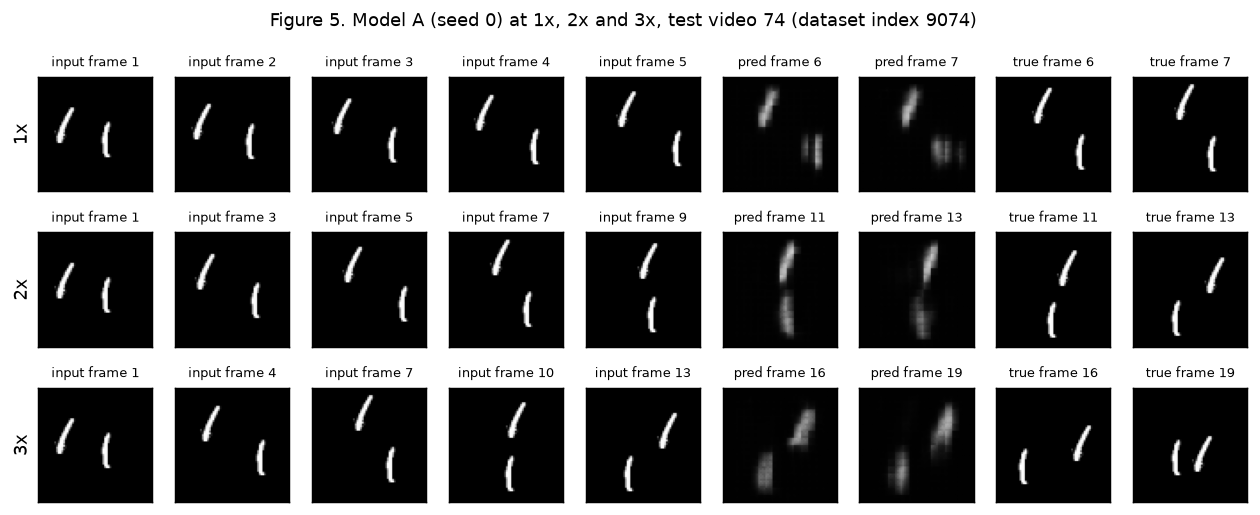
\includegraphics[width=\linewidth]{figures/fig5_speed.png}
\end{figure}

\subsection*{Q2.9}
\textbf{Model A falls apart at 2×.} Its \(E^{(2)}\) rises from 0.0188 at 1× to 0.0455 at 2× and 0.0530 at 3× (Table 4). Both are worse than predicting a blank frame (Blank \(E^{(2)}\) = 0.0425 at 2× and 0.0426 at 3×, Table 4), though still better than Copy-last (0.0661 and 0.0703). At 2× the model has already gone from beating Blank by more than half to doing worse than Blank.

\textbf{This does not match the reach estimate.} Q2.3 gives 8 px per step, and the typical 2× speed is 6.6 px/frame, inside that reach, so reach alone would predict that 2× is still manageable (this is also what I predicted in Q2.5). What the estimate misses is that reach is only an upper bound on what the network could connect. It says nothing about what it learned to do. Model A was trained only on speeds up to about 5 px/frame, so its learned update does not follow displacements larger than that, whatever the inputs show.

\textbf{What the failure looks like (Figure 5, test video 74: two 1s that stay at least about 7 px apart in every frame shown).} At 1× the predicted digits sit where the true ones are, just blurred: the upper 1 is predicted at column 25.0, row 16.5 against 25.0, 16.3 in the truth. At 2× and 3× the predicted digits stall. Measured by blob centroids, they move only 1--5 px away from their positions in the last input frame, while the true digits move 6--15 px. At 3× they barely move at all (under 2.5 px in both predicted frames), so frame 19 still shows the digits near where they were in frame 13, while the true digits have bounced and moved closer together. Both digits are also smeared into blobs. There are no duplicated digits, and nothing vanishes. Stalling suggests the model does not use the displacement it observed between input frames, which is larger than anything it was trained on, and falls back to keeping each digit close to its last position. Blurring suggests it is unsure where the digits are and hedges by spreading intensity over the possible positions.


\subsection*{Q2.10}
No.~Fast motion never appeared in training (Figure 1(b) has almost nothing above 5 px/frame), and it also approaches or exceeds the reach, so both explanations predict the failure we see, and model A alone cannot separate them. The 2× failure at 6.6 px/frame, inside the 8 px reach, points towards unfamiliar motion, but the reach is only an estimate of an upper bound, so this is not conclusive.

\textbf{Experiment.} Change one factor at a time:

\begin{enumerate}
\def\labelenumi{\arabic{enumi}.}
\item
  Train the same architecture (8 px reach) with speed augmentation, so 2× and 3× motion becomes familiar. If its 2× and 3× errors drop to near its 1× error, the failure was unfamiliar motion.
\item
  Train an architecture with a strictly larger reach on the same speed-augmented data. If it does clearly better at 3× than step 1, the remaining failure is architectural reach.
  (Optionally, also train the larger-reach model at 1× only; if it still fails at 2× and 3×, more reach without the data does not help.) Steps 1 and 2 are exactly models C and D.
\end{enumerate}


\newpage
\subsection*{4. What Can Data Fix?}
\subsection*{Q2.11}
\textit{(included exactly as first written)}

Model B (symmetry augmentation, 1× only) will shrink \(C_M\) and \(C_R\) and bring \(E_M\) and \(E_R\) close to \(E^{(5)}\), helping most on rotation because that gap comes mainly from unfamiliar digit appearance; it will not help at 2× or 3×. Model C (speed augmentation) will clearly reduce \(E^{(2)}\) at 2×, where about 6.6 px/frame is still inside model A's 8 px reach, but only partly at 3×, where most motion exceeds that reach, and it will leave the mirror and rotation gaps roughly as in model A. Model D (larger reach plus speed augmentation) will fix the remaining 3× failure, beating C at 3× while matching it at 1× and 2×, with consistency gaps similar to A's because it sees no symmetry augmentation.


\begin{table}[!htbp]\centering\footnotesize\setlength{\tabcolsep}{4pt}
\begin{tabular}{llllll}
\toprule
Model & $E^{(5)}$ & $C_M$ & $E_M$ & $C_R$ & $E_R$\\
\midrule
A & \makecell[l]{0.0222\\{\scriptsize(0.0227, 0.0216)}} & \makecell[l]{0.00193\\{\scriptsize(0.00199, 0.00187)}} & \makecell[l]{0.0228\\{\scriptsize(0.0234, 0.0222)}} & \makecell[l]{0.00317\\{\scriptsize(0.00318, 0.00316)}} & \makecell[l]{0.0239\\{\scriptsize(0.0244, 0.0234)}}\\
B & \makecell[l]{0.0221\\{\scriptsize(0.0224, 0.0217)}} & \makecell[l]{0.00150\\{\scriptsize(0.00143, 0.00156)}} & \makecell[l]{0.0221\\{\scriptsize(0.0225, 0.0218)}} & \makecell[l]{0.00160\\{\scriptsize(0.00159, 0.00162)}} & \makecell[l]{0.0221\\{\scriptsize(0.0223, 0.0219)}}\\
C & \makecell[l]{0.0271\\{\scriptsize(0.0268, 0.0274)}} & \makecell[l]{8.07e-04\\{\scriptsize(8.71e-04, 7.44e-04)}} & \makecell[l]{0.0273\\{\scriptsize(0.0270, 0.0276)}} & \makecell[l]{0.00198\\{\scriptsize(0.00212, 0.00185)}} & \makecell[l]{0.0281\\{\scriptsize(0.0279, 0.0284)}}\\
D & \makecell[l]{0.0274\\{\scriptsize(0.0276, 0.0272)}} & \makecell[l]{7.66e-04\\{\scriptsize(7.43e-04, 7.89e-04)}} & \makecell[l]{0.0276\\{\scriptsize(0.0278, 0.0274)}} & \makecell[l]{0.00186\\{\scriptsize(0.00167, 0.00204)}} & \makecell[l]{0.0285\\{\scriptsize(0.0285, 0.0284)}}\\
\bottomrule
\end{tabular}

\medskip
\begin{tabular}{lllllll}
\toprule
Model & $E^{(2)}$ 1$\times$ & $E^{(2)}$ 2$\times$ & $E^{(2)}$ 3$\times$ & params & train s/epoch & inference s\\
\midrule
A & \makecell[l]{0.0188\\{\scriptsize(0.0193, 0.0183)}} & \makecell[l]{0.0455\\{\scriptsize(0.0449, 0.0462)}} & \makecell[l]{0.0530\\{\scriptsize(0.0520, 0.0539)}} & 480{,}784 & \makecell[l]{47.3\\{\scriptsize(46.7, 47.8)}} & \makecell[l]{1.43\\{\scriptsize(1.43, 1.43)}}\\
B & \makecell[l]{0.0184\\{\scriptsize(0.0186, 0.0183)}} & \makecell[l]{0.0452\\{\scriptsize(0.0470, 0.0434)}} & \makecell[l]{0.0521\\{\scriptsize(0.0555, 0.0488)}} & 480{,}784 & \makecell[l]{46.7\\{\scriptsize(46.7, 46.7)}} & \makecell[l]{1.43\\{\scriptsize(1.43, 1.43)}}\\
C & \makecell[l]{0.0235\\{\scriptsize(0.0236, 0.0234)}} & \makecell[l]{0.0291\\{\scriptsize(0.0292, 0.0291)}} & \makecell[l]{0.0334\\{\scriptsize(0.0334, 0.0334)}} & 480{,}784 & \makecell[l]{46.9\\{\scriptsize(46.9, 47.0)}} & \makecell[l]{1.43\\{\scriptsize(1.43, 1.42)}}\\
D & \makecell[l]{0.0247\\{\scriptsize(0.0247, 0.0247)}} & \makecell[l]{0.0292\\{\scriptsize(0.0293, 0.0290)}} & \makecell[l]{0.0326\\{\scriptsize(0.0326, 0.0326)}} & 480{,}784 & \makecell[l]{52.7\\{\scriptsize(52.7, 52.7)}} & \makecell[l]{1.79\\{\scriptsize(1.80, 1.79)}}\\
\bottomrule
\end{tabular}
\caption{Models A-D (mean (seed 0, seed 1)); hardware: macOS-15.0-arm64-arm-64bit-Mach-O (mps)}
\end{table}

\subsection*{Q2.12}
\textbf{Model D} is model A with \textbf{dilation 2 in the second ConvLSTM layer} (3×3 kernel, padding 2). Everything else is identical to model A: 4×4 patch folding, 64 hidden channels in both layers, 3×3 kernels, the 1×1 output convolution, the 9-step rollout without teacher forcing, and the training protocol with speed augmentation (k drawn uniformly from \{1, 2, 3\}). Dilation adds no weights, so D has 480,784 parameters, the same as A and well under the 721,176 limit.

\textbf{Reach.} Same convention as Q2.3 (one grid cell = 4 px):

\begin{itemize}
\item
  the layer-1 convolution (3×3, dilation 1) moves information 1 cell;
\item
  the layer-2 convolution (3×3, dilation 2) samples cells 2 apart, so it moves information 2 cells;
\item
  the longest path, from \(u_\tau\) or \(h^{(1)}_{\tau-1}\) through both layers, is 1 + 2 = 3 cells = \textbf{12 px}; from \(h^{(2)}_{\tau-1}\) it is 2 cells = 8 px.
\end{itemize}

D's reach is 12 px along a row or column (\(3\sqrt{2} \times 4 \approx 17.0\) px diagonally), strictly larger than A's 8 px (11.3 px diagonally), and above the median 3× speed of 9.95 px/frame.

\textbf{How it was chosen (validation split only).} I compared three candidates: 5×5 kernels with 44 hidden channels (652,272 parameters, 16 px reach), dilation 2 in layer 2 (480,784 parameters, 12 px), and 8×8 patches (594,496 parameters, 16 px). In 5-epoch runs, both 16 px candidates stayed on the blank-frame plateau (validation \(E^{(5)}\) ≈ 0.0395 every epoch), while the dilated model kept improving. I re-ran dilation and 8×8 patches for 15 epochs (dropping 5×5 kernels, which took about 120 s per epoch against 59 s). The 8×8 model was still stuck at 0.0395, while the dilated model reached validation \(E^{(2)}\) of 0.0278, 0.0313 and 0.0340 at 1×, 2× and 3×, so I chose dilation. Training is slightly slower than A (52.7 s against 47.3 s per epoch) because the dilated convolution is less efficient on the GPU.


\subsection*{Q2.13}
\begin{itemize}
\item
  \textbf{Mirror and rotation gaps: appearance.} Model B changes only the training orientation of the digits (same architecture, same 1× motion), and it removes the gap: \(E_M\) = 0.0221 and \(E_R\) = 0.0221, equal to its \(E^{(5)}\) of 0.0221, against A's \(E_M\) = 0.0228 and \(E_R\) = 0.0239 with \(E^{(5)}\) = 0.0222. \(C_R\) halves from 0.00317 to 0.00160. Models C and D, which see no new orientations, keep a rotation gap (\(E_R\) − \(E^{(5)}\) = 0.00102 for both, against 3.87e-05 for B). \(C_T\) alone would be misleading here: C and D have lower \(C_M\) than B (8.07e-04 and 7.66e-04 against 0.00150), partly because their predictions are blurrier (Q2.6 and Q2.14).
\item
  \textbf{Speed failure (2× and 3×): unfamiliar motion.} Model C has exactly A's architecture and reach (8 px) and only adds speed augmentation, and it fixes most of the failure: \(E^{(2)}\) at 2× drops from 0.0455 to 0.0291 and at 3× from 0.0530 to 0.0334, both now well below Blank (0.0425 at 2× and 0.0426 at 3×, Table 4).
\item
  \textbf{Architectural reach: at most a small part of the 3× failure.} Model D adds reach (12 px) on top of C's data. At 2× it matches C (0.0292 against 0.0291), and at 3× it is only slightly better (0.0326 against 0.0334, the same gap for both seeds).
\end{itemize}

So the case in the question, where C still does badly at 3× and D does well, did not happen here. If it had, it would have meant that the data had taught C everything about fast motion it could use, and that the remaining error came from the architecture. More data cannot fix that, because training changes the weights but not which positions are connected: if a digit's new position is more than the reach away from its old one, no path in that step's computation links the two, whatever the weights are.

C coped with 3× (about 10 px/frame) despite an 8 px reach, probably for two reasons. A digit is about 20 px wide, so after a 10 px shift its old and new footprints still overlap, and the edges the network has to connect are within 8 px of each other. The model can also carry velocity in its hidden state across the five input steps rather than relying on one update. The reach is a bound on a single point, not a hard limit for an extended object.


\subsection*{Q2.14}
\textbf{Symmetry augmentation (B) cost nothing:} \(E^{(5)}\) at 1× is 0.0221 against A's 0.0222.

\textbf{Speed augmentation did cost 1× accuracy:} \(E^{(5)}\) rises from 0.0222 to 0.0271 for C (+22\%) and 0.0274 for D (+23\%), and \(E^{(2)}\) at 1× from 0.0188 to 0.0235 (C) and 0.0247 (D). Both seeds agree. Two likely causes: with the same 30 epochs, only about a third of the training windows are at 1×, and one network now has to cover a much wider range of speeds, so its 1× predictions are blurrier (compare Figure 6b's 1× row with Figure 5's).

\textbf{It was worth it for this question's goal.} In exchange, \(E^{(2)}\) drops by about 36\% at 2× (0.0455 to 0.0291) and 37\% at 3× (0.0530 to 0.0334), and the model goes from worse than Blank to clearly better than Blank at those speeds, while staying well ahead of Blank and Copy-last at 1×. If the model will only ever see 1× clips, model A or B is the better choice.


\newpage
\subsection*{5. The Final Model}
\textbf{Choice of final model.} I wrapped model D (symmetrised D) and did not train D+B. Table 5 shows that what symmetry augmentation buys (B's transformed errors matching its \(E^{(5)}\)) is exactly what symmetrisation guarantees by construction (\(E_M\) = \(E_R\) = \(E^{(5)}\), shown below), so D+B would add about an hour of training for, at most, the small accuracy gain that symmetrised B shows over B (\(E^{(5)}\) 0.0214 against 0.0221). It is possible that D+B would be slightly more accurate after wrapping, because its eight predictions would agree more before averaging; I did not test this.

\textbf{Proof that the symmetrised forecaster has \(C_M\) = \(C_R\) = 0.} Write \(\bar f(X) = \frac18\sum_{g\in G} g^{-1} f(gX)\). Take any \(h \in G\). Then

\[\bar f(hX) = \frac18\sum_{g\in G} g^{-1} f(ghX).\]

\(G\) is a group, so as \(g\) runs over \(G\), \(g' = gh\) also runs over every element of \(G\) exactly once. Substituting \(g = g'h^{-1}\), so that \(g^{-1} = h\,g'^{-1}\):

\[\bar f(hX) = \frac18\sum_{g'\in G} h\,g'^{-1} f(g'X) = h\Big(\frac18\sum_{g'\in G} g'^{-1} f(g'X)\Big) = h\,\bar f(X).\]

The middle step holds because \(h\) only rearranges pixels, so it is linear and can be taken out of the average. \(M\) and \(R\) are both in \(G\), so \(\bar f(MX) = M\bar f(X)\) and \(\bar f(RX) = R\bar f(X)\) for every input. Therefore \(C_M = C_R = 0\) exactly, for any \(f\). Table 6 gives values of about 1e-16, which is floating-point rounding.

The same argument gives \(E_T = \mathrm{MSE}(\bar f(TX), TY) = \mathrm{MSE}(T\bar f(X), TY) = \mathrm{MSE}(\bar f(X), Y) = E^{(5)}\), since rearranging pixels does not change a mean squared error. This is why \(E_M\), \(E_R\) and \(E^{(5)}\) are identical in Table 6.

\begin{table}[!htbp]\centering\footnotesize\setlength{\tabcolsep}{4pt}
\begin{tabular}{llllll}
\toprule
Model & $E^{(5)}$ & $C_M$ & $E_M$ & $C_R$ & $E_R$\\
\midrule
sym B & \makecell[l]{0.0214\\{\scriptsize(0.0217, 0.0212)}} & \makecell[l]{8.72e-17\\{\scriptsize(9.13e-17, 8.31e-17)}} & \makecell[l]{0.0214\\{\scriptsize(0.0217, 0.0212)}} & \makecell[l]{7.02e-17\\{\scriptsize(7.33e-17, 6.71e-17)}} & \makecell[l]{0.0214\\{\scriptsize(0.0217, 0.0212)}}\\
sym D & \makecell[l]{0.0274\\{\scriptsize(0.0276, 0.0272)}} & \makecell[l]{5.56e-17\\{\scriptsize(5.58e-17, 5.53e-17)}} & \makecell[l]{0.0274\\{\scriptsize(0.0276, 0.0272)}} & \makecell[l]{4.32e-17\\{\scriptsize(4.38e-17, 4.26e-17)}} & \makecell[l]{0.0274\\{\scriptsize(0.0276, 0.0272)}}\\
\bottomrule
\end{tabular}

\medskip
\begin{tabular}{lllllll}
\toprule
Model & $E^{(2)}$ 1$\times$ & $E^{(2)}$ 2$\times$ & $E^{(2)}$ 3$\times$ & params & train s/epoch & inference s\\
\midrule
sym B & \makecell[l]{0.0180\\{\scriptsize(0.0181, 0.0178)}} & \makecell[l]{0.0443\\{\scriptsize(0.0463, 0.0424)}} & \makecell[l]{0.0511\\{\scriptsize(0.0546, 0.0476)}} & 480{,}784 & \makecell[l]{46.7\\{\scriptsize(46.7, 46.7)}} & \makecell[l]{11.4\\{\scriptsize(11.8, 11.1)}}\\
sym D & \makecell[l]{0.0247\\{\scriptsize(0.0247, 0.0246)}} & \makecell[l]{0.0292\\{\scriptsize(0.0294, 0.0291)}} & \makecell[l]{0.0325\\{\scriptsize(0.0325, 0.0325)}} & 480{,}784 & \makecell[l]{52.7\\{\scriptsize(52.7, 52.7)}} & \makecell[l]{13.9\\{\scriptsize(13.9, 14.0)}}\\
\bottomrule
\end{tabular}
\caption{Symmetrised forecasters; training time is that of the underlying model.}
\end{table}

\begin{figure}[!htbp]\centering
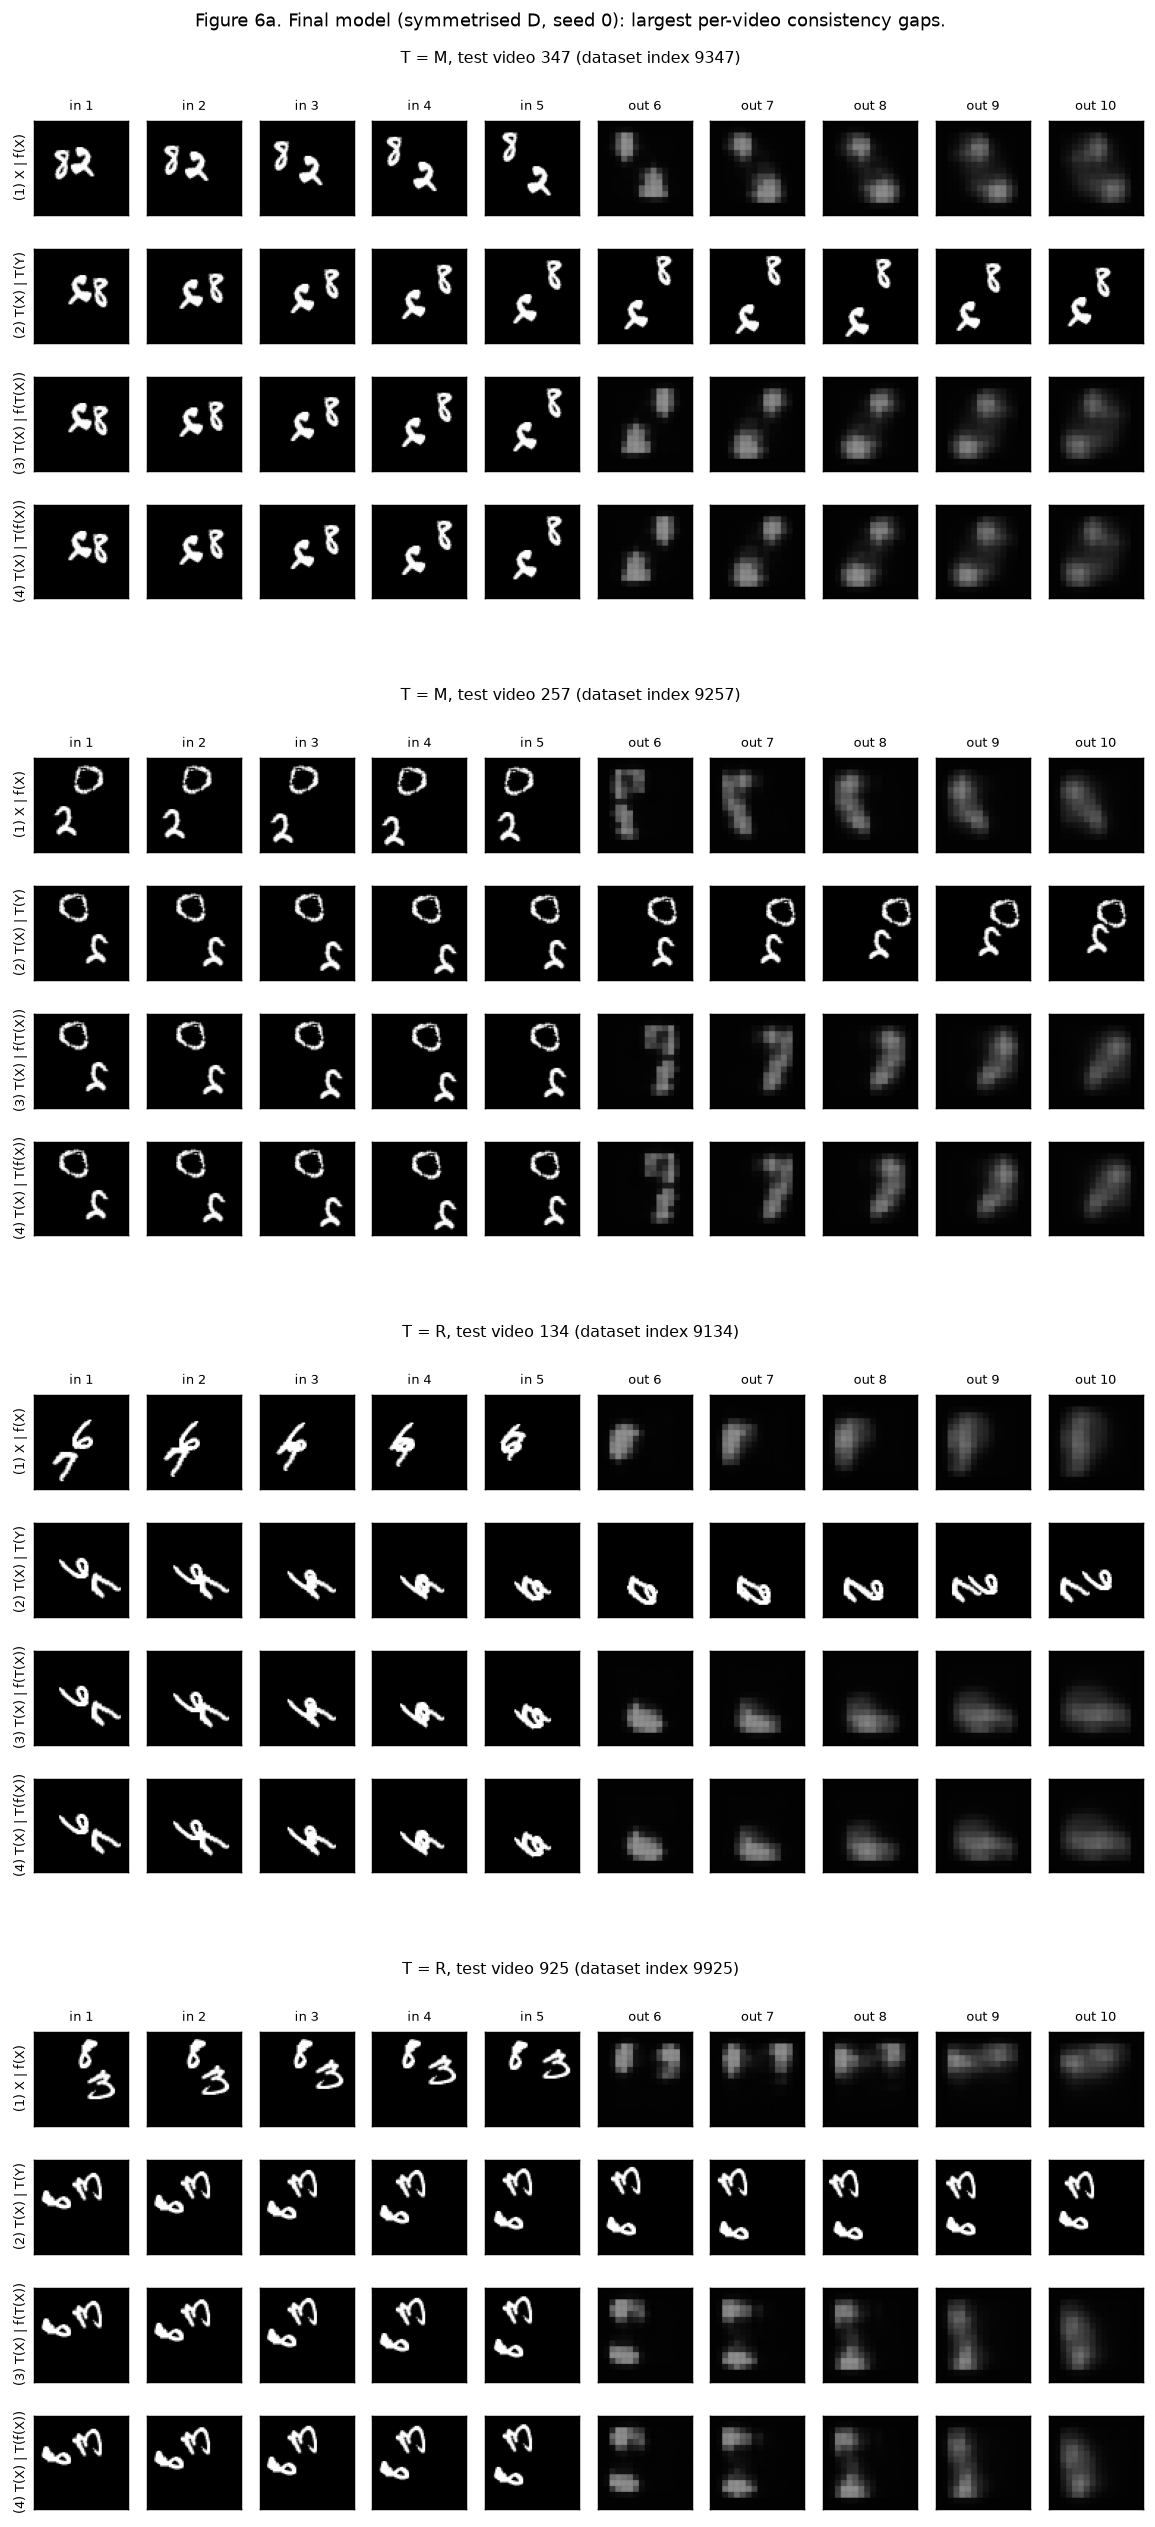
\includegraphics[height=0.82\textheight]{figures/fig6a_consistency.png}
\caption*{\footnotesize GIFs: \texttt{Question2/results/gifs/fig6a\_M\_video257.gif}, \texttt{Question2/results/gifs/fig6a\_M\_video347.gif}, \texttt{Question2/results/gifs/fig6a\_R\_video134.gif}, \texttt{Question2/results/gifs/fig6a\_R\_video925.gif}}
\end{figure}

\begin{figure}[!htbp]\centering
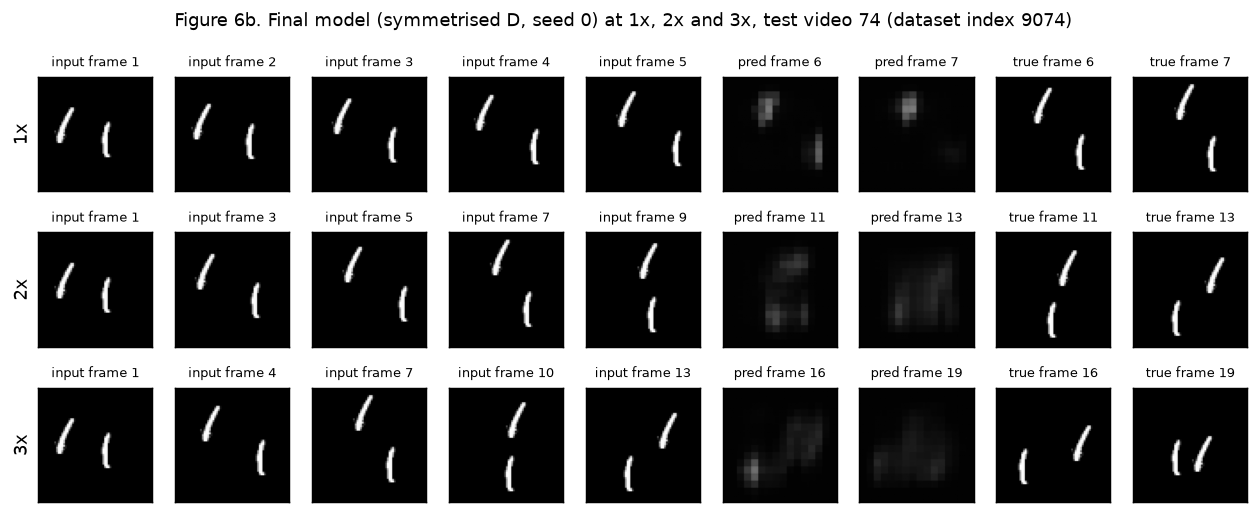
\includegraphics[width=\linewidth]{figures/fig6b_speed.png}
\end{figure}

\subsection*{Q2.15}
\begin{itemize}
\item
  \textbf{Consistency.} Learned symmetry is approximate: model B reduces A's gaps but leaves \(C_M\) = 0.00150 and \(C_R\) = 0.00160. Built-in symmetry is exact: symmetrised B has \(C_M\) = 8.72e-17 and \(C_R\) = 7.02e-17, and symmetrised D 5.56e-17 and 4.32e-17. Built-in symmetry is exact because of the group argument above: it holds for any weights, while augmentation only encourages the weights towards consistency on the training distribution.
\item
  \textbf{Accuracy.} Wrapping did not hurt here. Symmetrised B improves on B everywhere: \(E^{(5)}\) 0.0214 against 0.0221, \(E^{(2)}\) 0.0443 against 0.0452 at 2× and 0.0511 against 0.0521 at 3×. Symmetrised D matches D on the original clips (\(E^{(5)}\) 0.0274 for both, \(E^{(2)}\) 0.0247, 0.0292 and 0.0325 against 0.0247, 0.0292 and 0.0326) and improves the transformed clips (\(E_R\) 0.0274 against 0.0285, \(E_M\) 0.0274 against 0.0276). For any symmetrised model, the transformed errors equal \(E^{(5)}\) exactly.
\item
  \textbf{Inference cost.} Built-in symmetry costs eight forward passes: 11.4 s against 1.43 s for B, and 13.9 s against 1.79 s for D (about 8× slower). Learned symmetry costs nothing at test time; it moves the cost into training.
\end{itemize}

\textbf{When averaging hurts.} Averaging eight predictions blurs the output when the eight disagree. That happens when the base model is much worse on some orientations than others (for example model A, trained only on upright digits: its rotated predictions are worse, and averaging mixes them into the good one), or when the data is not really symmetric (gravity, text, a camera that always faces one way). Here both B and D already had small gaps (B because it was trained on all eight orientations, D because its predictions are smooth), so averaging acted more like a small ensemble than a source of blur.


\subsection*{Q2.16}
\textbf{Partly.} For test video 925 under rotation, rows 3 and 4 of Figure 6a are now identical (per-video \(C_R\) drops from 0.00683 for model A to about 7e-17), so the final model's account of the scene no longer depends on its orientation. But it is the wrong account in both rows: the two digits still blur together into one vertical smear by frames 9--10, which is what model A did only in row 3, while in the truth they stay apart. The per-video \(E_R\) is 0.0389 against model A's 0.0357.

\begin{itemize}
\item
  \textbf{Symmetrisation} fixed the disagreement between rows 3 and 4. It also lowered this video's error relative to plain D (\(E_R\) 0.0389 against 0.0417).
\item
  \textbf{Model D's changes} (larger reach and speed augmentation) were not aimed at this failure: the digits here barely move, so neither reach nor speed is the problem, and speed augmentation made D's 1× predictions blurrier, which is why the final model's frames 9--10 are smoother than model A's.
\end{itemize}

The remaining failure, keeping two close digits apart, is not fixed by any of the changes.


\subsection*{Q2.17}
Partly. The final model learned a motion rule that holds across the speeds it was trained on, but it does not keep digits sharp or separate. The best evidence is speed: model A was worse than Blank at 2× and 3× (\(E^{(2)}\) 0.0455 and 0.0530 against 0.0425 and 0.0426), while the final model beats both references at every speed (0.0247, 0.0292 and 0.0325). Its exact consistency proves little, since \(C_T\) = 0 and \(E_T\) = \(E^{(5)}\) hold by construction for any symmetrised model. Better evidence: the unwrapped D's transformed errors were already close to its \(E^{(5)}\) without symmetry augmentation (\(E_M\) = 0.0276 and \(E_R\) = 0.0285, against 0.0274). A skeptic should next see newly generated Moving MNIST videos at a speed outside the training range. One test it still fails: in video 925 (Figure 6a) it merges two nearby digits into one streak.


\newpage
%=====================================================================
\section*{Use of Generative AI}
I used Claude Code (Anthropic, Claude Opus 5.5). 
I used it to understand the tasks and how should I approach them.
I used it to draw diagrams
I used it for scaffolding the tasks code and drafting the LaTeX report.

\section*{References}
\begin{itemize}
\item Shi, X., Chen, Z., Wang, H., Yeung, D.-Y., Wong, W.-K., and Woo, W.\ (2015). Convolutional LSTM Network:
A Machine Learning Approach for Precipitation Nowcasting. NeurIPS.
\item Cho, K., van Merri\"enboer, B., Gulcehre, C., Bahdanau, D., Bougares, F., Schwenk, H., and Bengio, Y.\ (2014).
Learning Phrase Representations using RNN Encoder--Decoder for Statistical Machine Translation. EMNLP.
\item Farneb\"ack, G.\ (2003). Two-Frame Motion Estimation Based on Polynomial Expansion. SCIA.
\item Srivastava, N., Mansimov, E., and Salakhutdinov, R.\ (2015). Unsupervised Learning of Video Representations
using LSTMs. ICML.
\item Zeng, A., Chen, M., Zhang, L., and Xu, Q.\ (2023). Are Transformers Effective for Time Series Forecasting? AAAI.
\end{itemize}

\end{document}
